\documentclass[11pt]{article}
\usepackage[utf8]{inputenc}
\usepackage[spanish]{babel}
\decimalpoint
\usepackage{amsmath}
\usepackage{amsthm}
\usepackage{amssymb}
\usepackage{graphicx}
\usepackage[margin=0.8in]{geometry}
\usepackage{fancyhdr}
\usepackage[inline]{enumitem}
\usepackage{float}
\usepackage{cancel}
\usepackage{bigints}
\usepackage{listings}
\usepackage{xcolor}
\usepackage{listingsutf8}
\usepackage{algpseudocode}
\usepackage{algorithm}
\usepackage{apacite}
\usepackage{tcolorbox}
\usepackage{multicol}
\usepackage{tipa}
\usepackage{caption} 
\pagestyle{fancy}
\usepackage{hyperref}
\usepackage{mathtools}% http://ctan.org/pkg/mathtools
\renewcommand{\labelenumii}{\theenumii}
\renewcommand{\theenumii}{\theenumi.\arabic{enumii}.}
\hypersetup{
    colorlinks,
    citecolor=black,
    filecolor=black,
    linkcolor=black,
    urlcolor=black
}
\newcommand{\xvdash}[1]{%
	\vdash^{\mkern-10mu\scriptscriptstyle\rule[-.9ex]{0pt}{0pt}#1}%
}
\setlength{\headheight}{15pt} 
\lhead{Tarea 11. Respaldo y restauración de una máquina virtual en la nube}
\rhead{\thepage}
\lfoot{ESCOM-IPN}
\renewcommand{\footrulewidth}{0.5pt}
\setlength{\parskip}{0.5em}
\newcommand{\ve}[1]{\overrightarrow{#1}}
\newcommand{\abs}[1]{\left\lvert #1 \right\lvert}
\newcommand{\blank}{\text{\textcrb}}
\date{\today}
\title{Tarea 11. Respaldo y restauración de una máquina virtual en la nube}
\author{Sanchez Mendez Edmundo Josue}

\lstset{
tabsize = 4, %% set tab space width
showstringspaces = false, %% prevent space marking in strings, string is defined as the text that is generally printed directly to the console
numbers = left, %% display line numbers on the left
commentstyle = \color{green}, %% set comment color
keywordstyle = \color{blue}, %% set keyword color
stringstyle = \color{red}, %% set string color
rulecolor = \color{black}, %% set frame color to avoid being affected by text color
basicstyle = \small \ttfamily , %% set listing font and size
breaklines = true, %% enable line breaking
numberstyle = \tiny,
}

\bibliographystyle{apacite}
\begin{document}
		\begin{titlepage}
			\begin{center}
				
				% Upper part of the page. The '~' is needed because \\
				% only works if a paragraph has started.
				
				\noindent
				\begin{minipage}{0.5\textwidth}
					\begin{flushleft} \large
						
\includegraphics[width=0.5\textwidth]{resources/ipn.png}
					\end{flushleft}
				\end{minipage}%
				\begin{minipage}{0.55\textwidth}
					\begin{flushright} \large
						
\includegraphics[width=0.5\textwidth]{resources/escom.png}
					\end{flushright}
				\end{minipage}
				
				\textsc{\LARGE Instituto Politécnico Nacional}\\[0.5cm]
				
				\textsc{\Large Escuela Superior de Cómputo}\\[1cm]
				
				% Title
				
				{ \huge Tarea 11. Respaldo y restauración de una máquina virtual en la nube \\[1cm] }
				
				{ \Large Unidad de aprendizaje: Desarrollo de Sistemas Distribuidos} \\[1cm]
				
				{ \Large Grupo: 4CV11 } \\[1cm]
				
				\noindent
				\begin{minipage}{0.5\textwidth}
					\begin{flushleft} \large
						\emph{Alumno:} \\
						Sanchez Mendez Edmundo Josue
					\end{flushleft}
				\end{minipage}%
				\begin{minipage}{0.5\textwidth}
					\begin{flushright} \large
						\emph{Profesor:} \\
						Pineda Guerrero Carlos 
					\end{flushright}
				\end{minipage}
				
				\vfill
				% Bottom of the page
				{\large {\today}}
			\end{center}
		\end{titlepage}
	
	\titlepage
	\tableofcontents
	\newpage
	
	\section{Introducción}
	Se deberá crear una máquina virtual en la nube de Azure y realizar los siguientes procedimientos que vimos en clase:
		\begin{enumerate}
			\item Habilitar el respaldo de la máquina virtual.
			\item Iniciar un respaldo completo.
			\item Restaurar la máquina virtual.
			\item Eliminar el proceso de respaldo.
		\end{enumerate}
	\section{Desarrollo}
		\subsection{Creación de la maquina virtual}
En esta parte veremos la creación de la maquina virtual sobre la cual realizaremos todos los procedimientos que se vieron en clase.
		\begin{figure}[H]
			\centering
			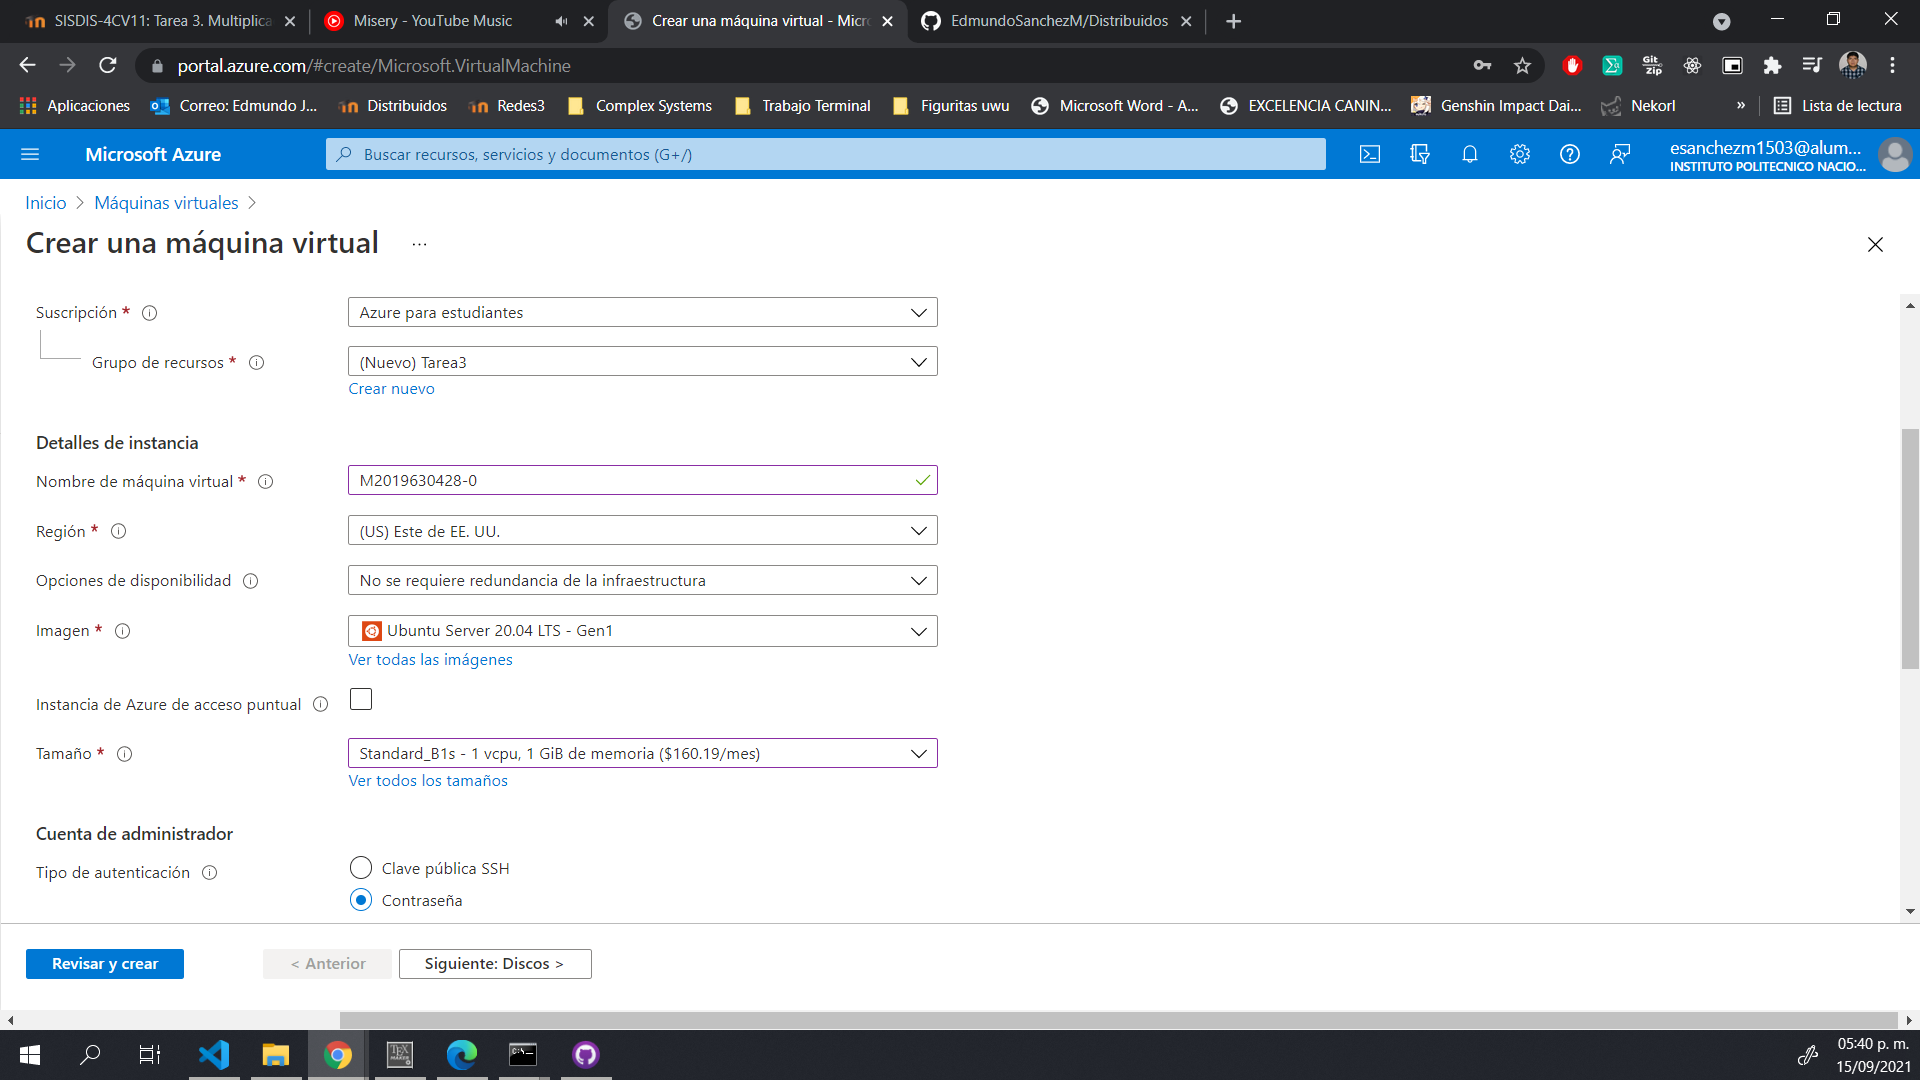
\includegraphics[scale=0.34]{resources/datosbasicos.png}
			\caption{Datos básicos de la maquina virtual.}\label{fig:picture}
		\end{figure}
		\begin{figure}[H]
			\centering
			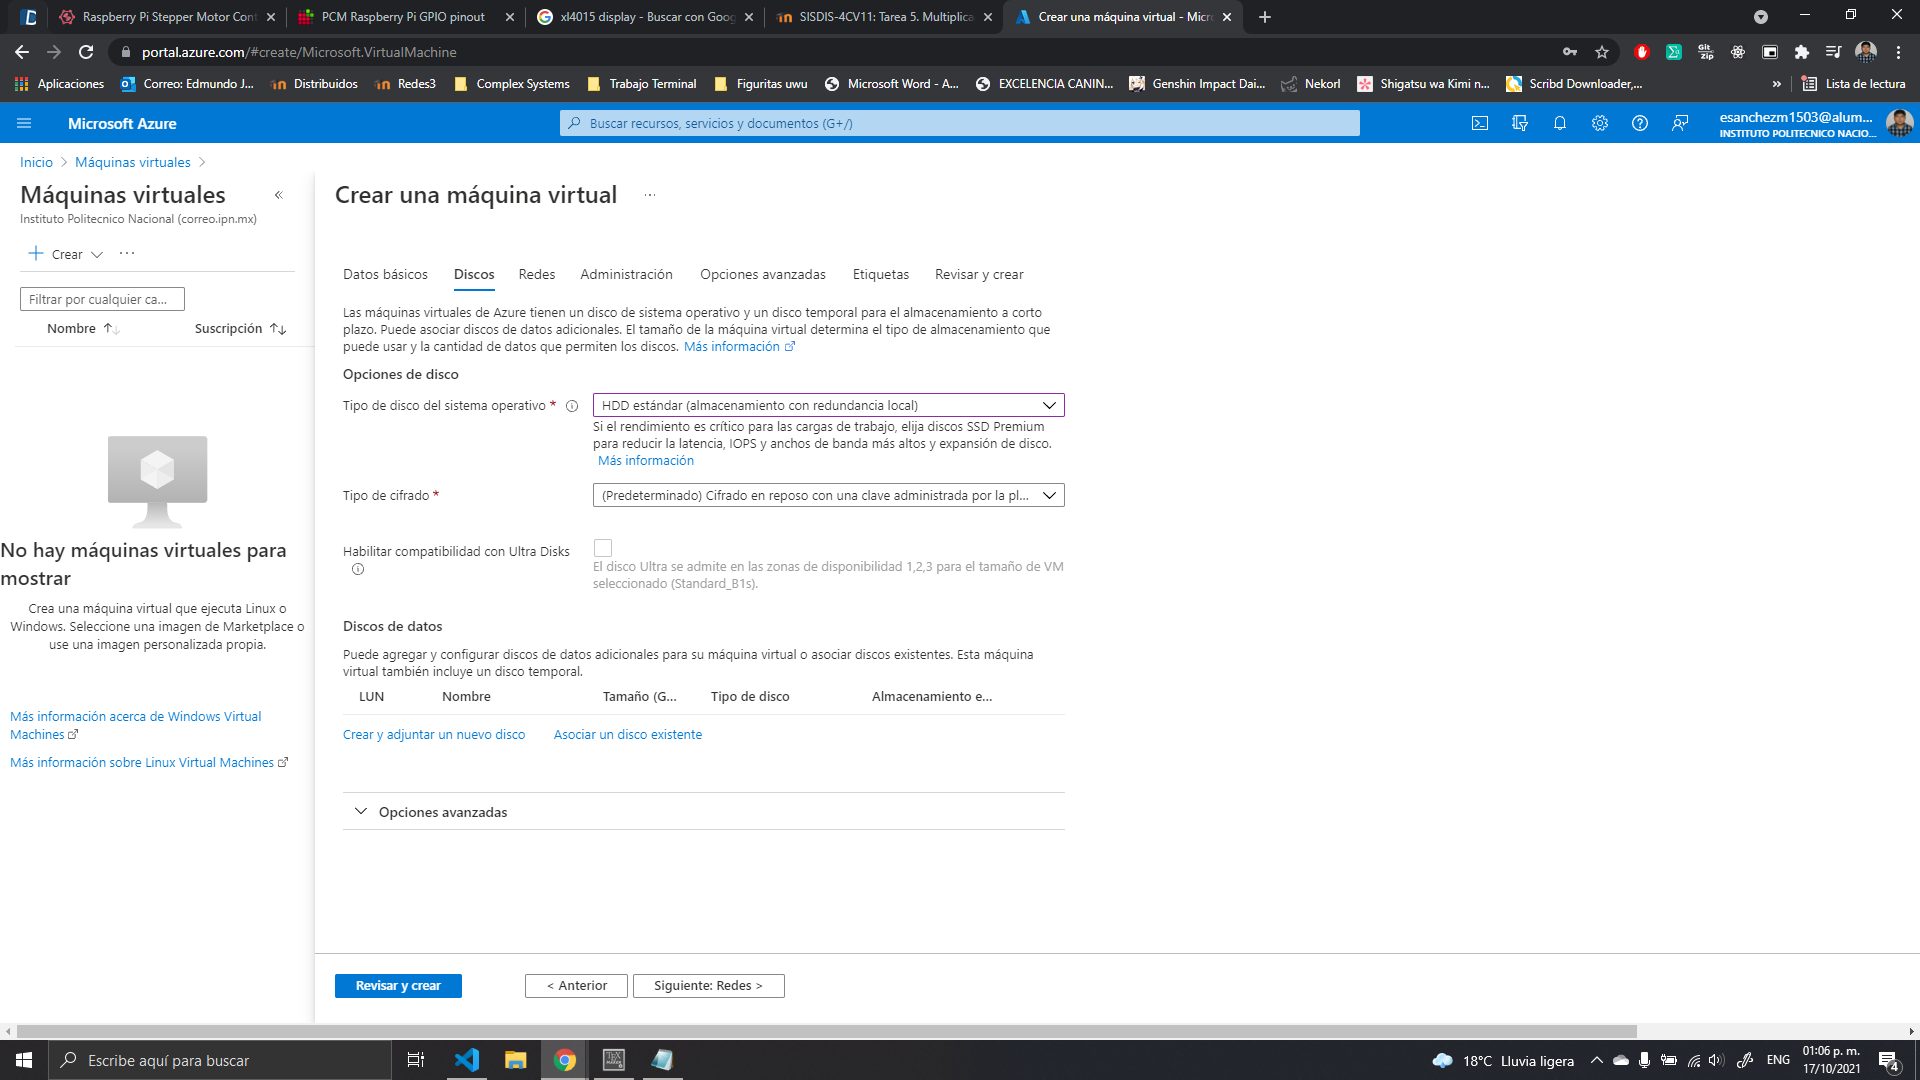
\includegraphics[scale=0.34]{resources/datosdisco.png}
			\caption{Configuración del tipo de disco de la maquina virtual.}\label{fig:picture}
		\end{figure}
		\begin{figure}[H]
			\centering
			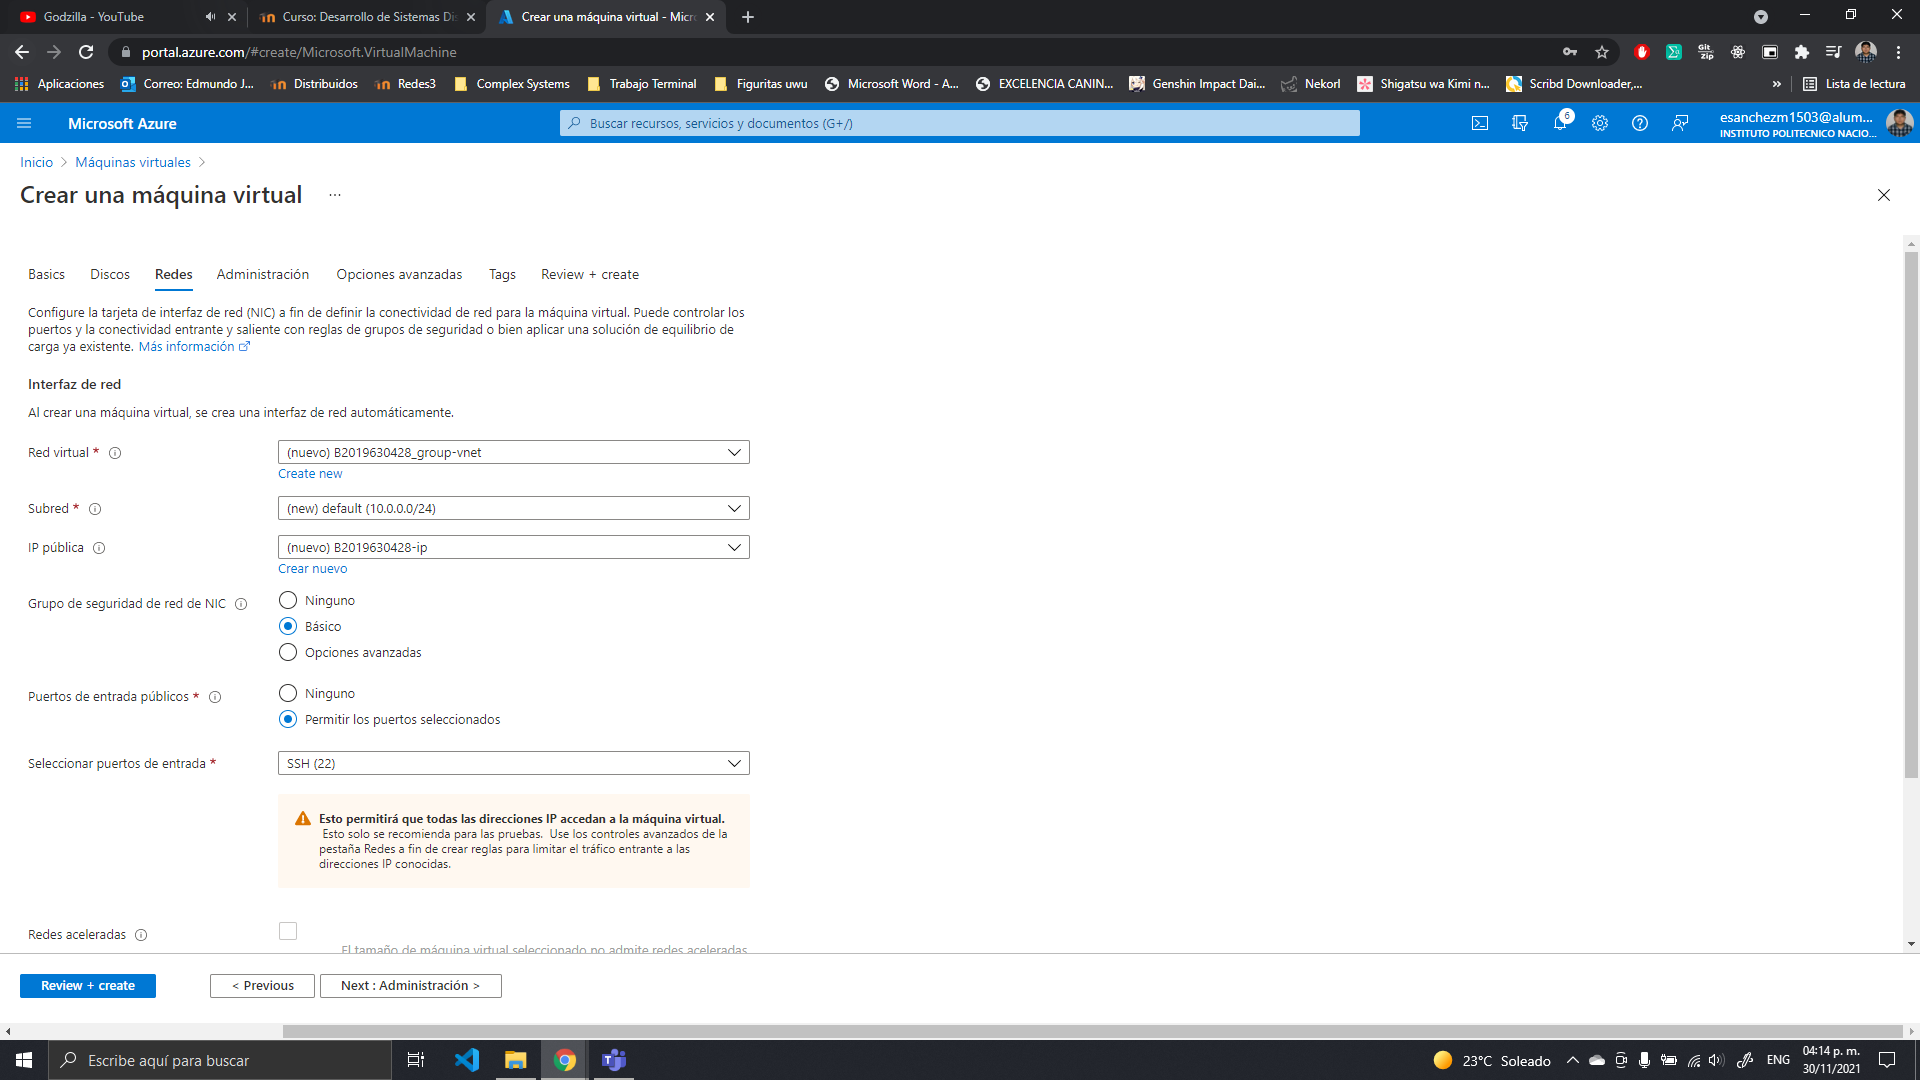
\includegraphics[scale=0.34]{resources/datosredes.png}
			\caption{Información sobre la redes de la maquina virtual.}\label{fig:picture}
		\end{figure}
		\begin{figure}[H]
			\centering
			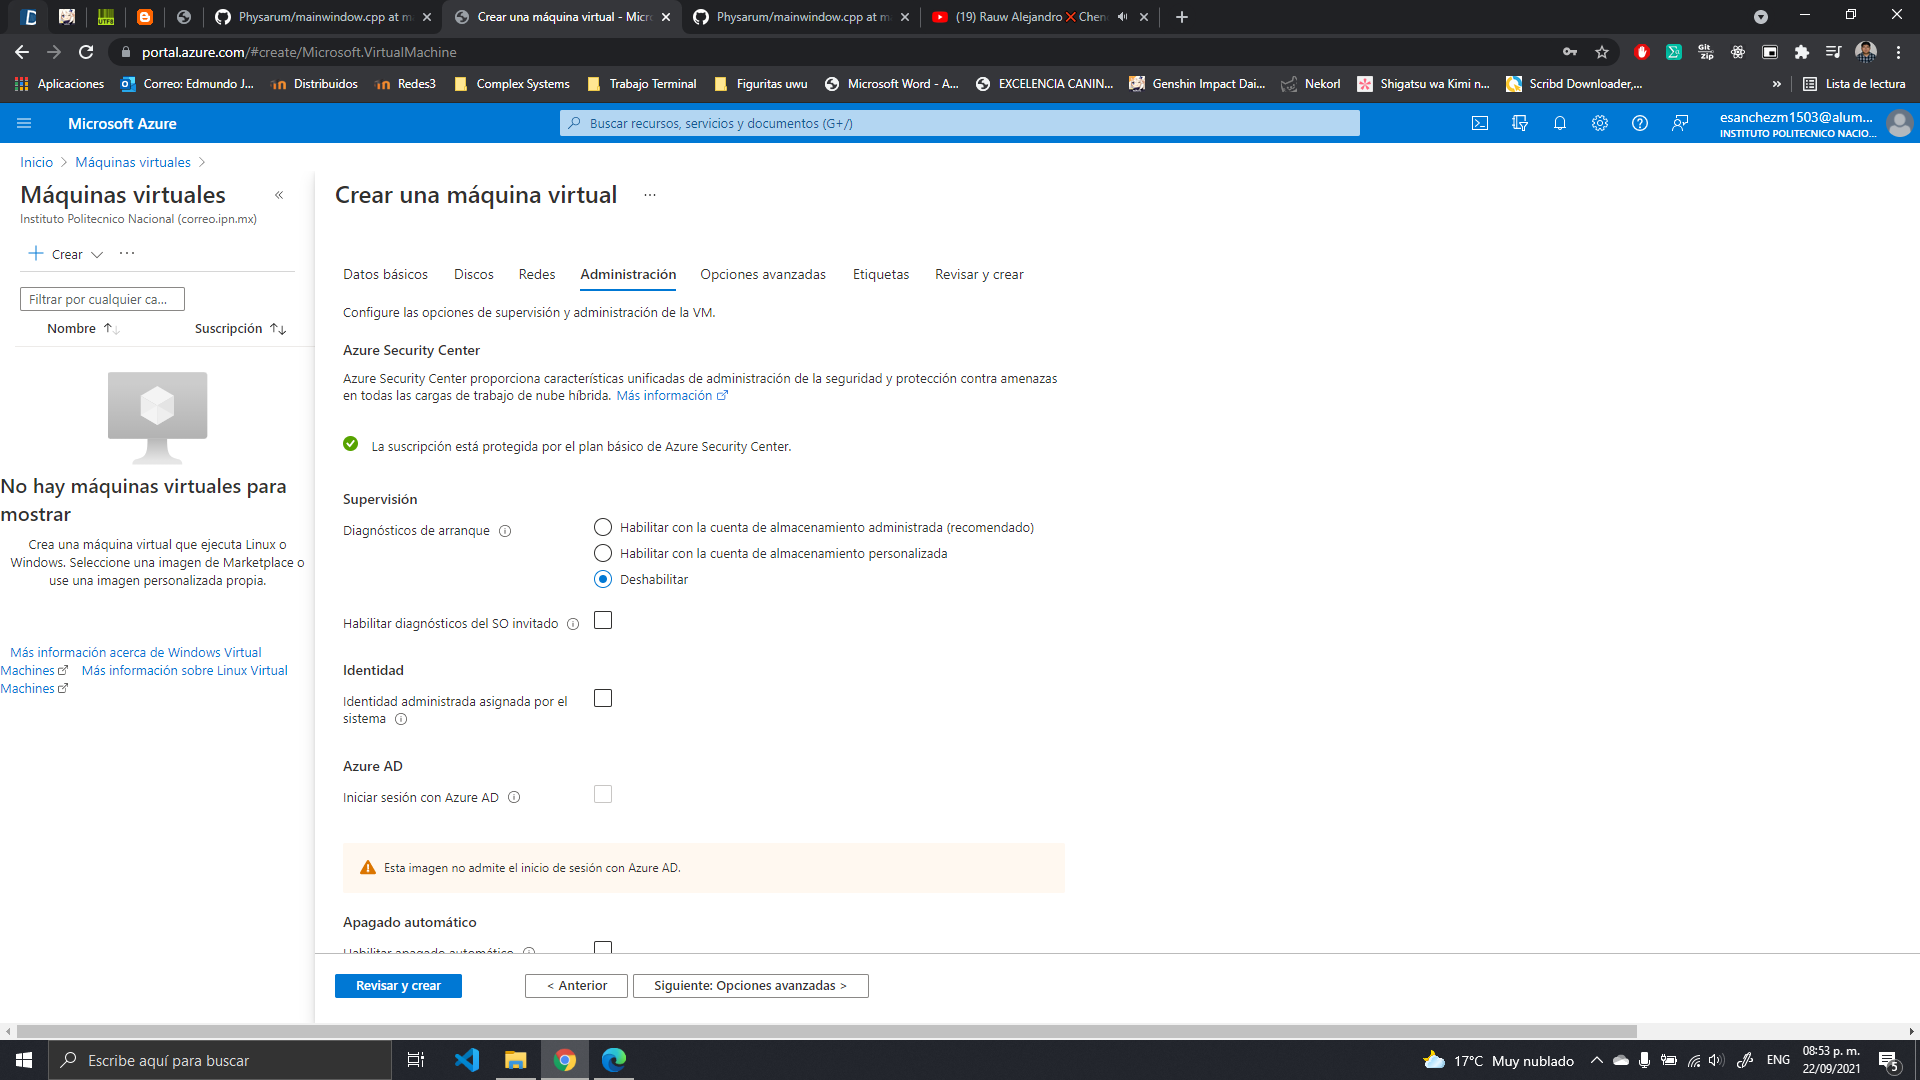
\includegraphics[scale=0.34]{resources/datosadministracion.png}
			\caption{Configuración de la administración de la maquina virtual.}\label{fig:picture}
		\end{figure}
		\begin{figure}[H]
			\centering
			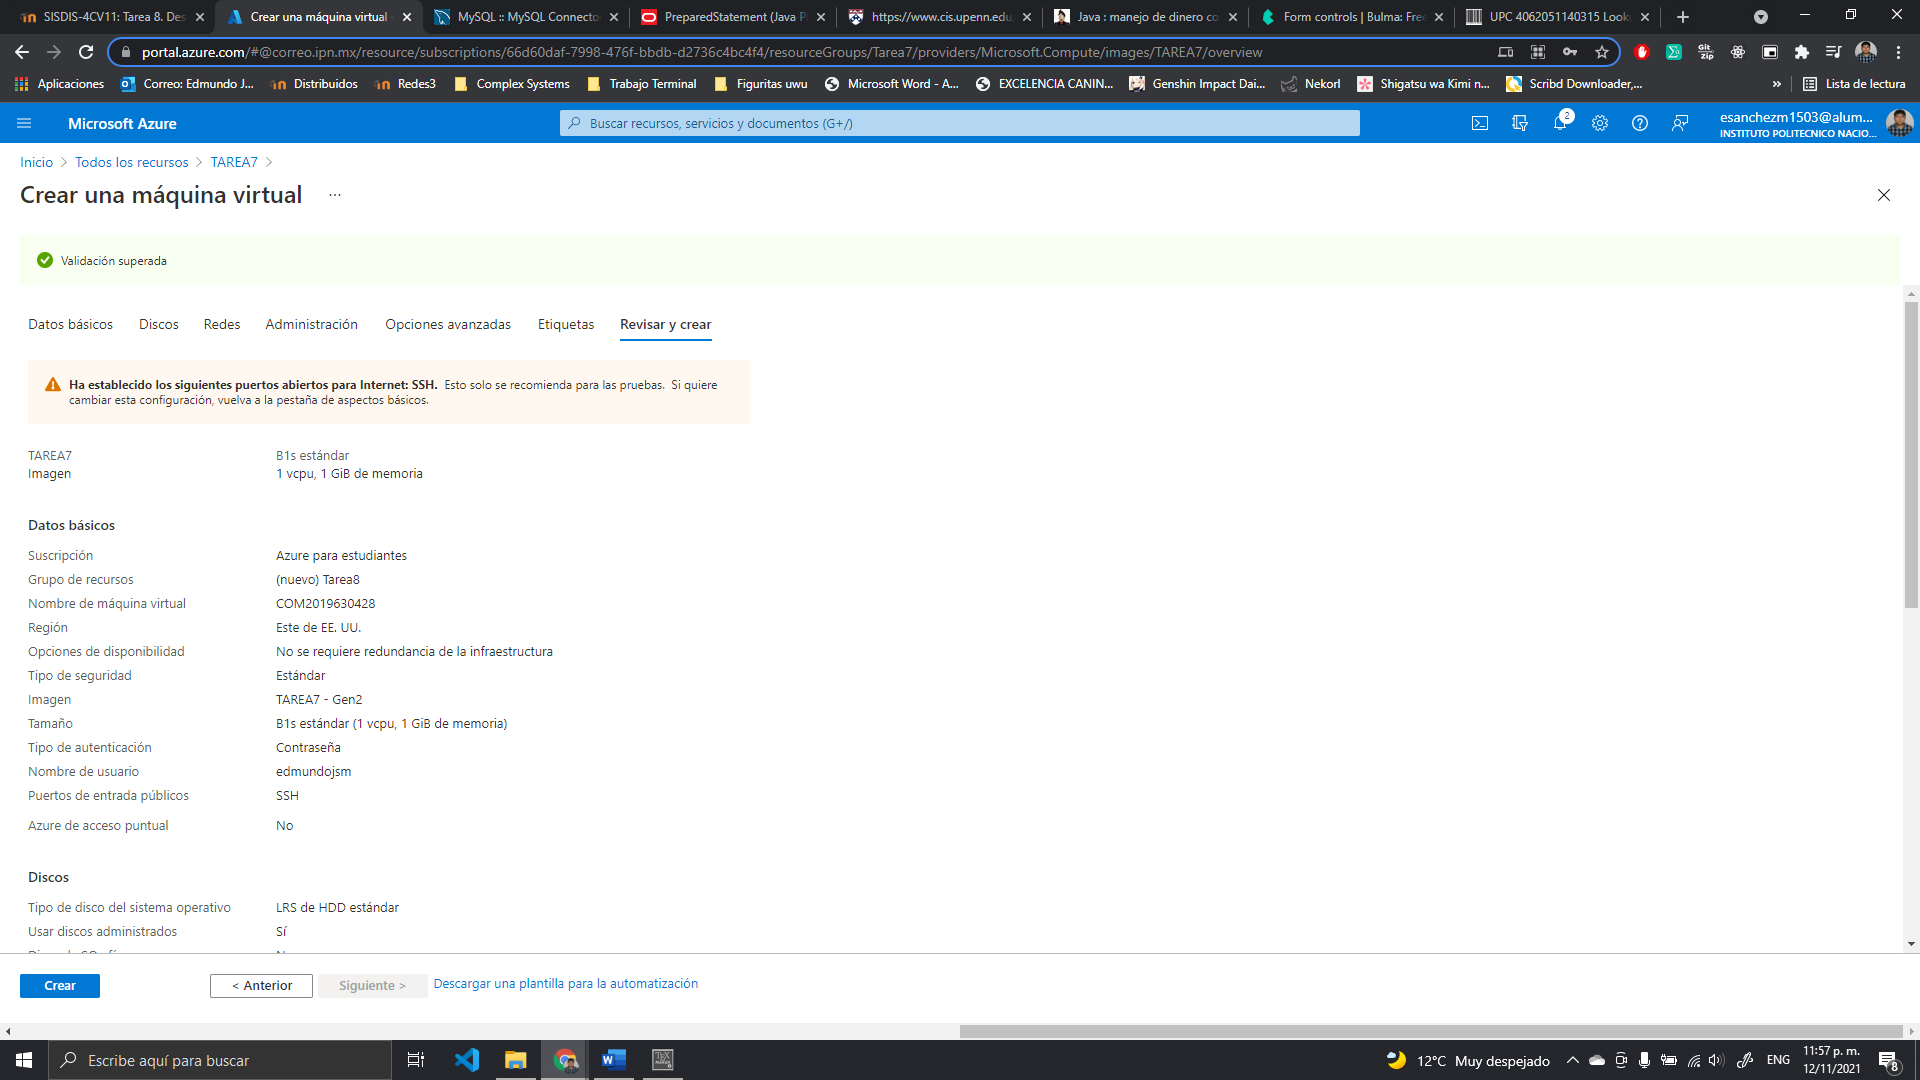
\includegraphics[scale=0.34]{resources/revisarycrear.png}
			\caption{Creación de la maquina virtual.}\label{fig:picture}
		\end{figure}
		\begin{figure}[H]
			\centering
			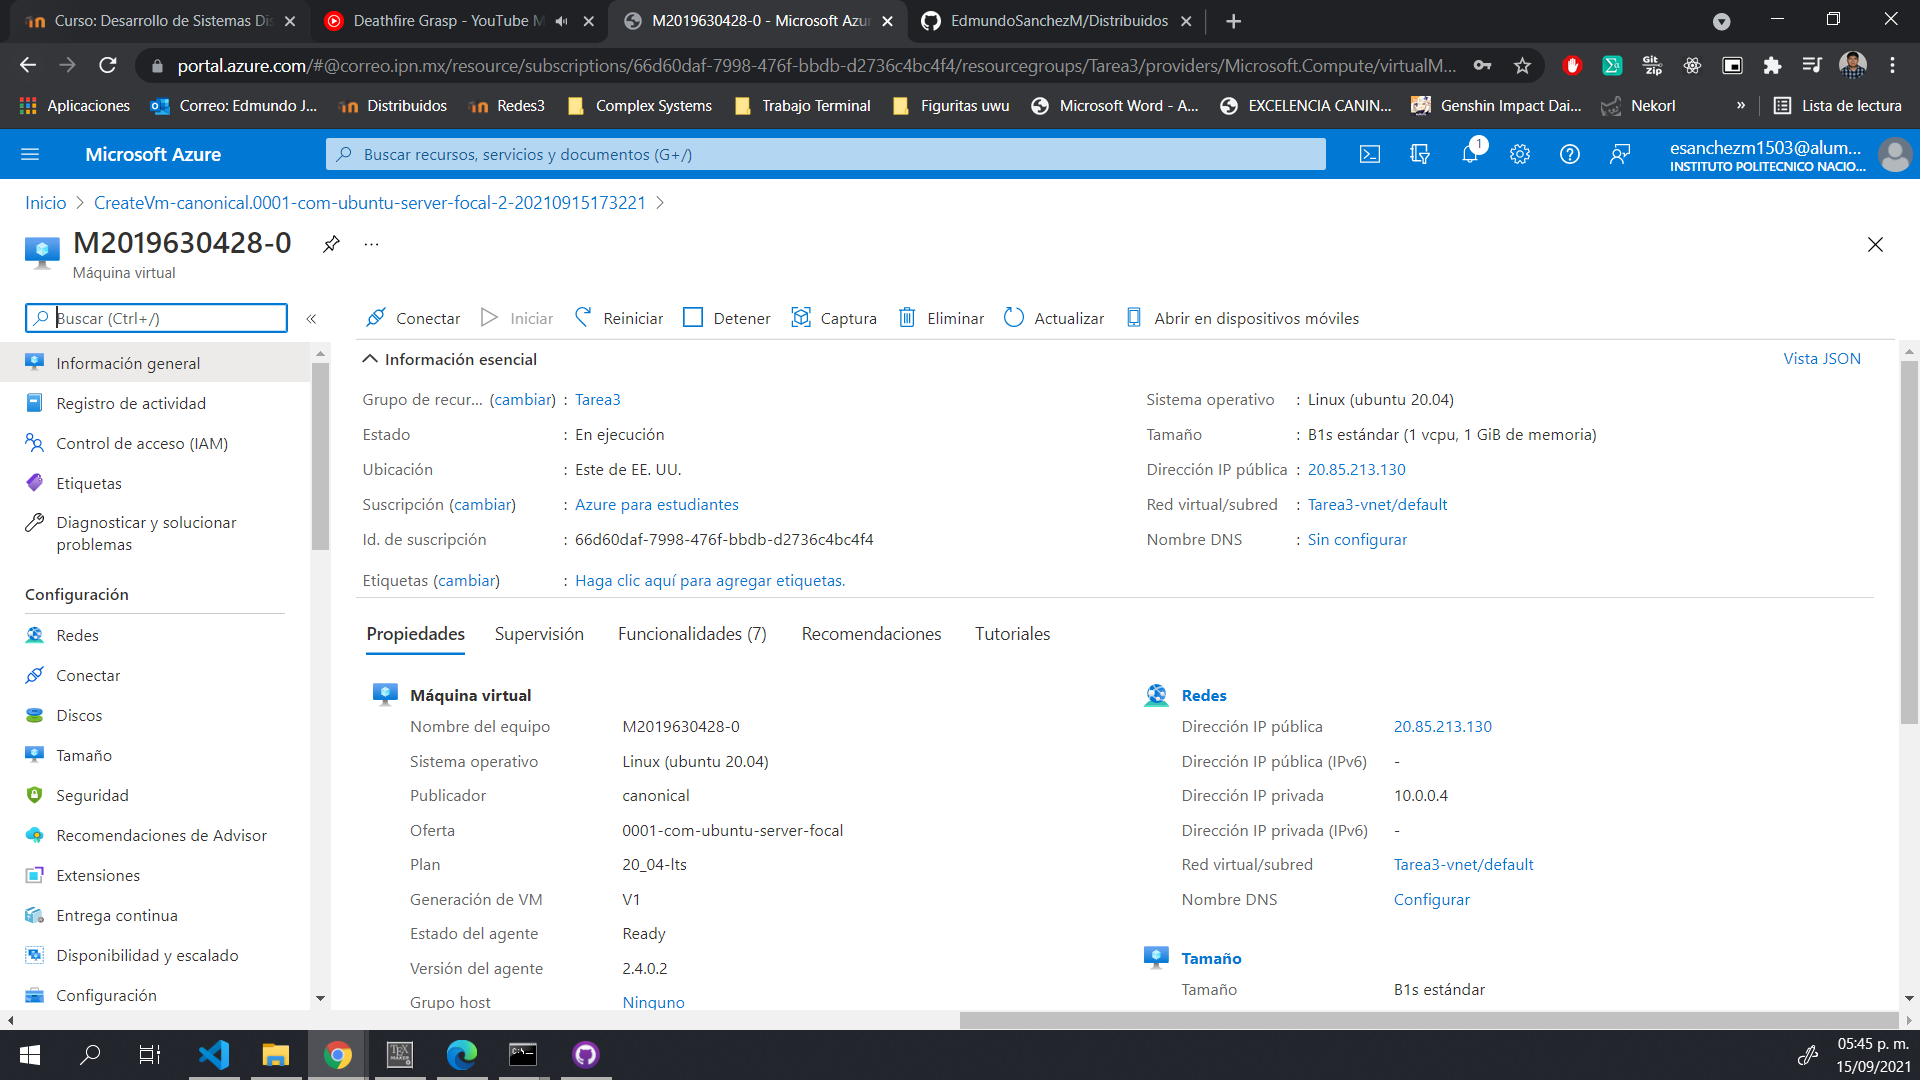
\includegraphics[scale=0.34]{resources/Panelcontrol.png}
			\caption{Panel de control de la maquina virtual.}\label{fig:picture}
		\end{figure}
		
		\subsection{Habilitar el respaldo de la máquina virtual}
		En esta parte veremos la forma de habilitar el respaldo en una maquina virtual de Azure. Para ello iremos a la maquina virtual deseada para realzar el respaldo, una vez ahí iremos al apartado ``Backup'' en el menú de operaciones, aquí crearemos un almacén de Recovery Services, para ello necesitamos introducir el grupo de recursos en donde se colocara el almacén, después debemos seleccionar la política de respaldo, por omisión DailyPolicy, o dar clic en ``Crear una nueva directiva'' para crear una nueva política de respaldo (Si la creamos se puede definir la frecuencia de respaldo (diario o semanal), la hora en la que se realizará el respaldo y el tiempo que se conservará los puntos de restauración.) Finalmente vente hay que darle clic al botón ``Habilitar Backup'', todo esto lo podemos ver en  la figura 7.
		\begin{figure}[H]
			\centering
			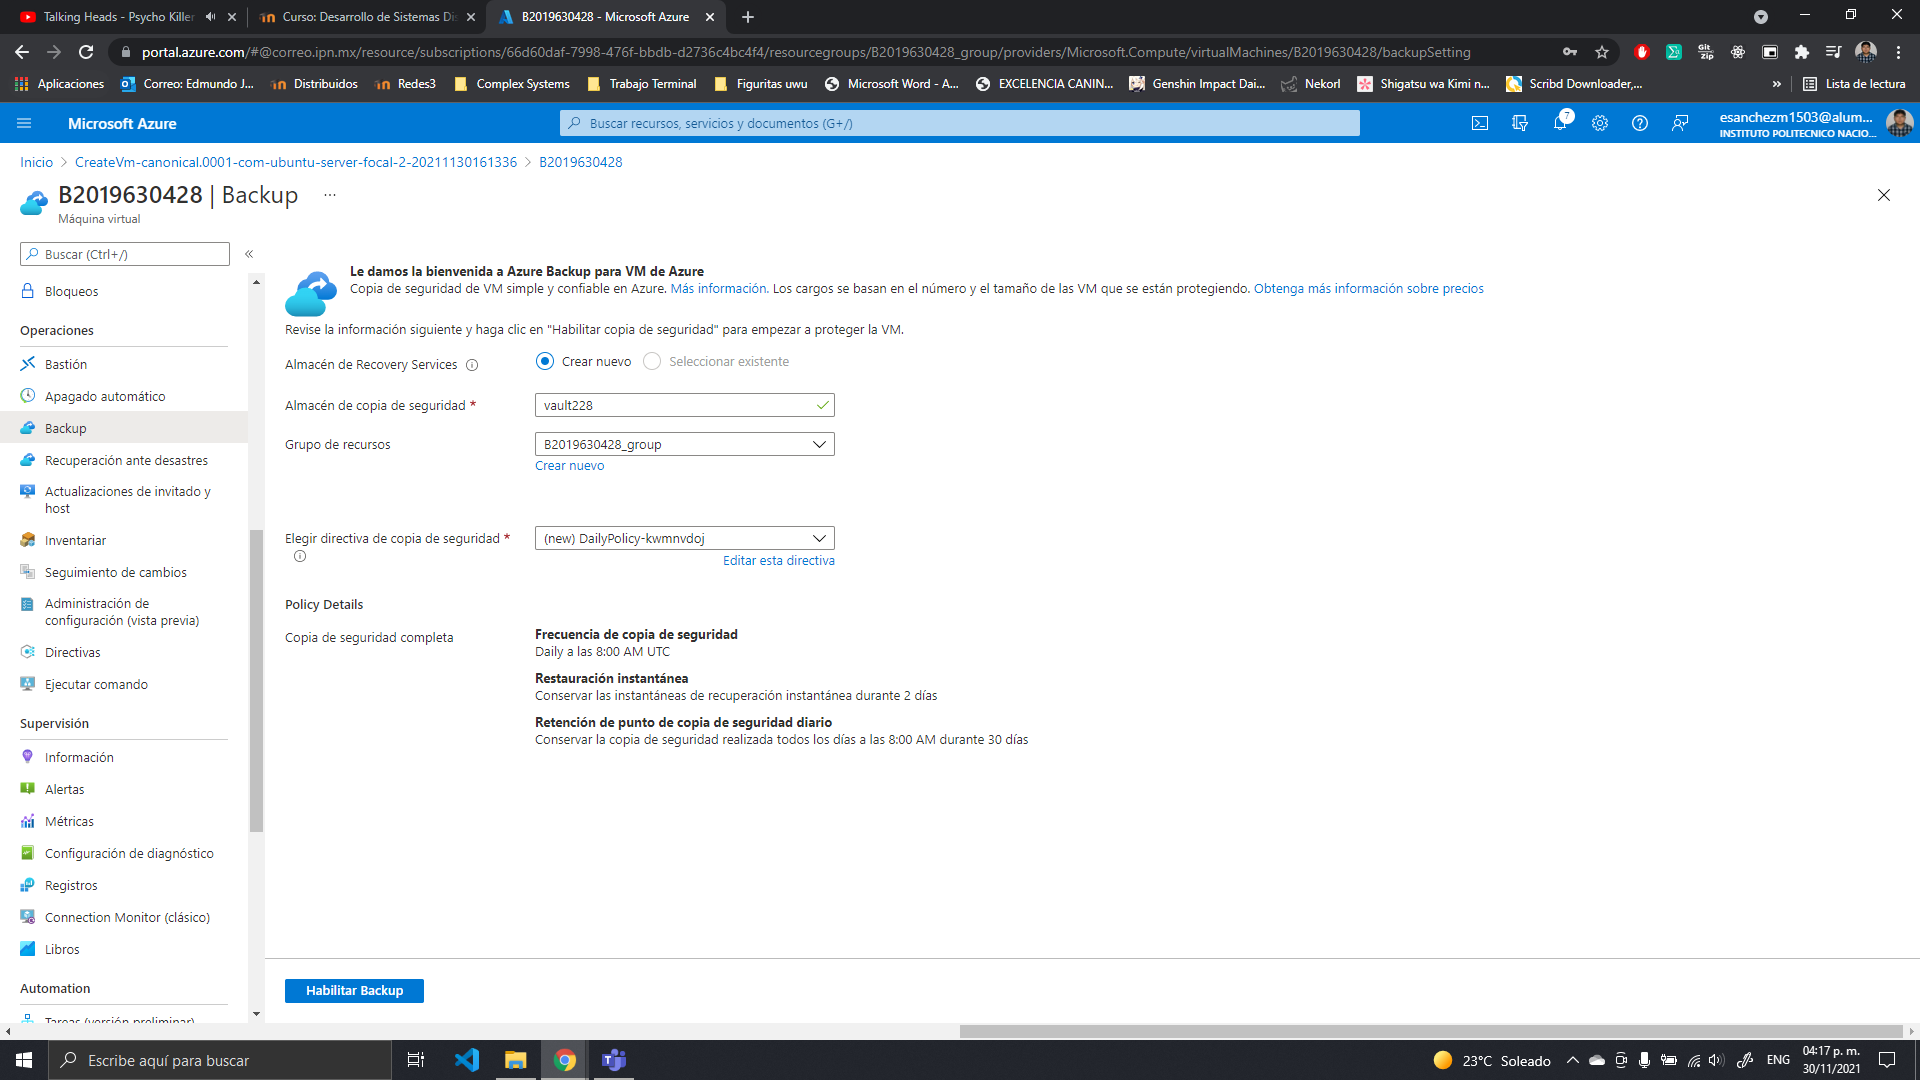
\includegraphics[scale=0.34]{resources/1.F.png}
			\caption{Habilitar el respaldo de una maquina virtual.}\label{fig:picture}
		\end{figure}
		Finalmente en la figura 8 podemos ver como la implementación del proceso de respaldo se realizo de manera correcta.
		\begin{figure}[H]
			\centering
			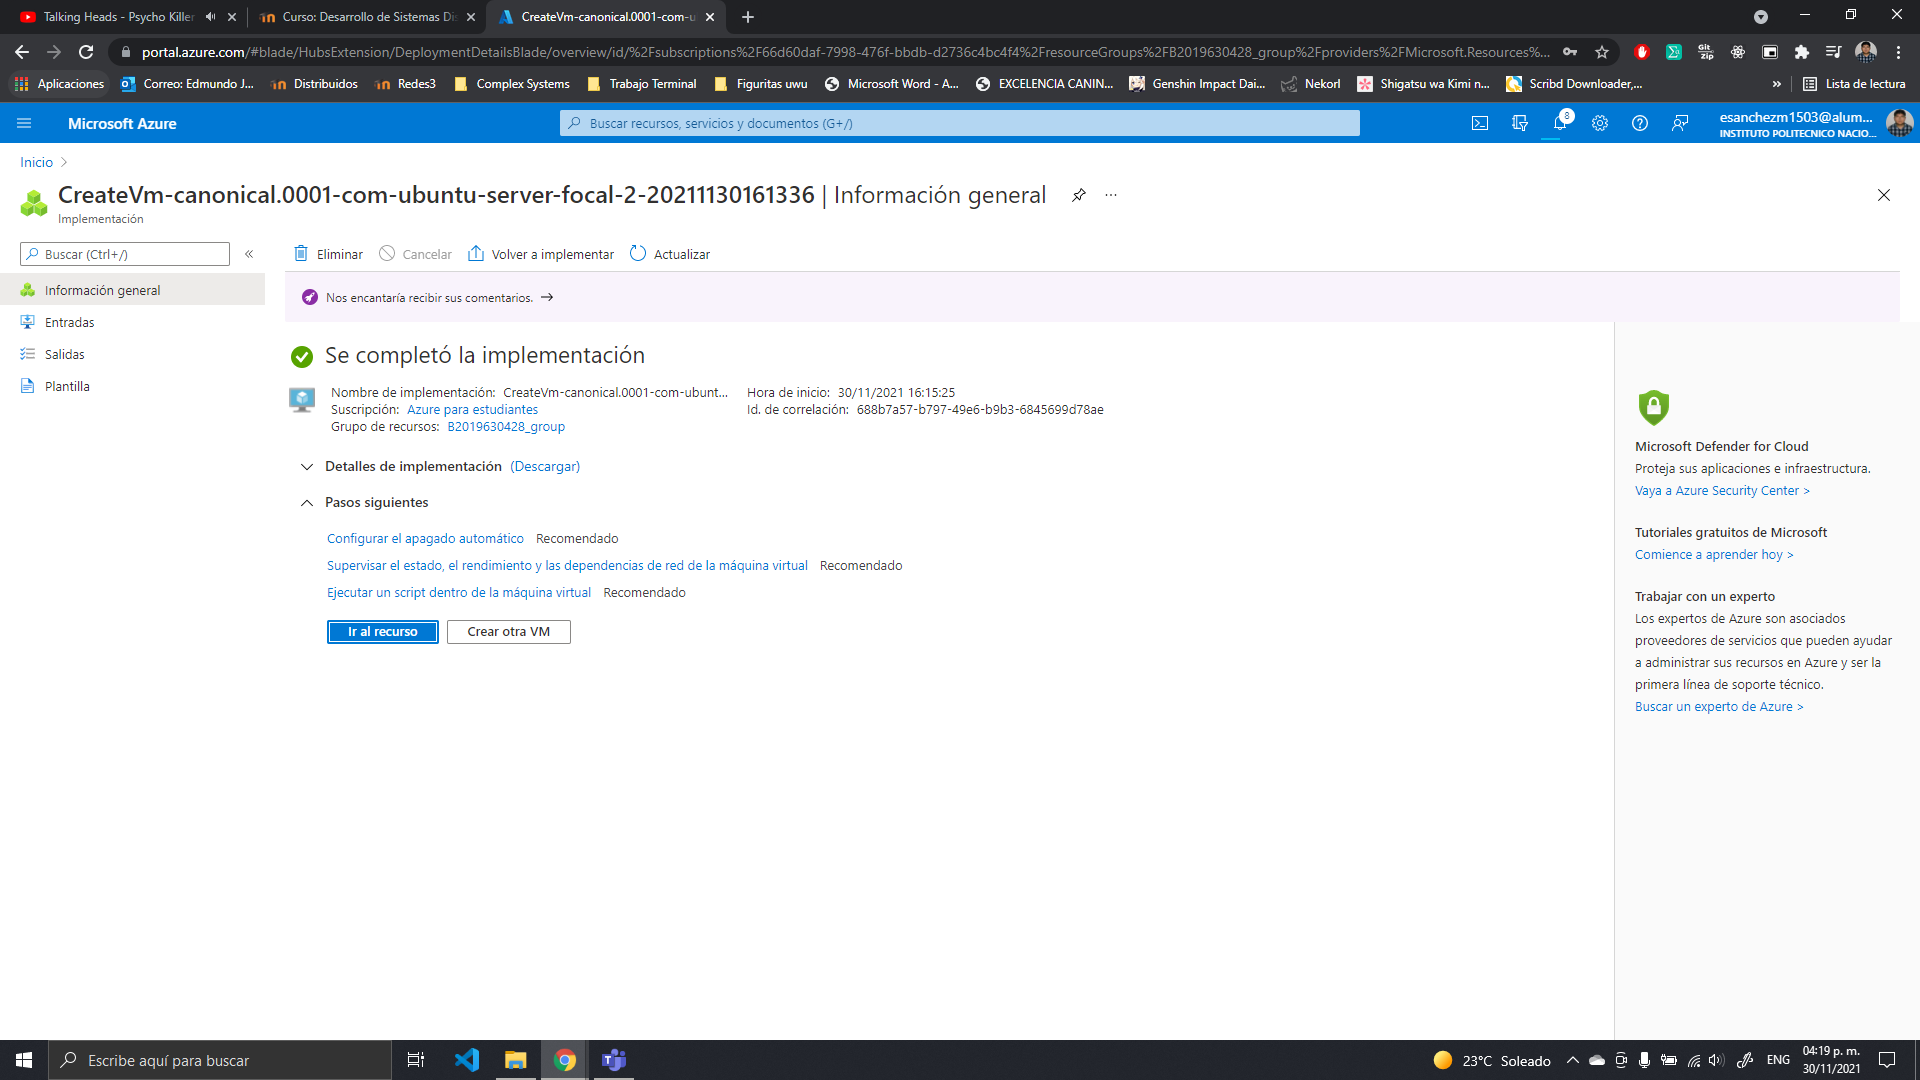
\includegraphics[scale=0.34]{resources/1.3.png}
			\caption{Implementación realizada de manera exitosa.}\label{fig:picture}
		\end{figure}
		\subsection{Iniciar un respaldo completo}
		Anteriormente vimos cómo habilitar un proceso de respaldo (backup job) para realizar un respaldo diario de una máquina virtual completa a cierta hora del día. Para iniciar el respaldo completo, debemos ir al panel de control de la maquina virtual y luego ir a la sección de ``Backup'' como vemos en la figura 9, de hecho si comparamos la figura 9 con la 7 hay un cambio en cuanto al contenido
		\begin{figure}[H]
			\centering
			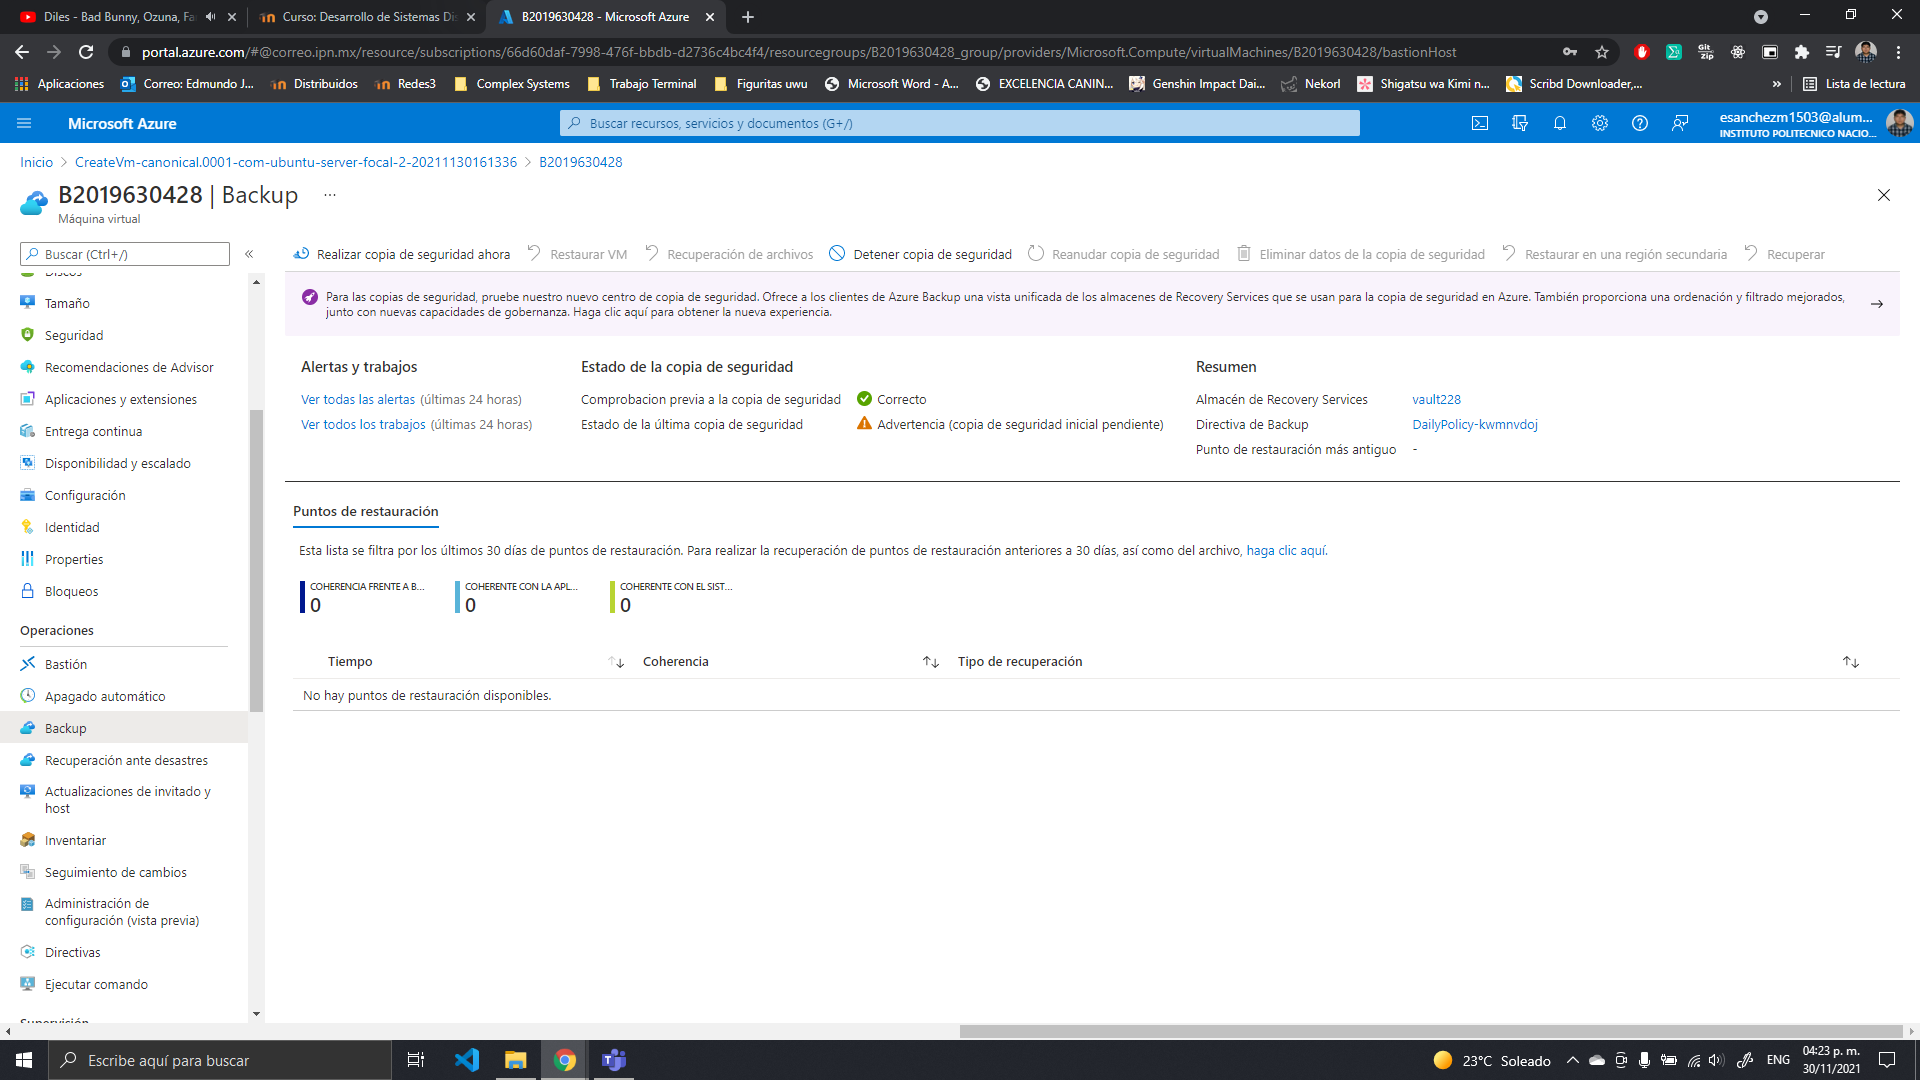
\includegraphics[scale=0.34]{resources/2.1.png}
			\caption{Opción ``Backup'' dentro de la maquina virtual.}\label{fig:picture}
		\end{figure}
		Una vez ahí seleccionaremos la opción ``Realizar copia de seguridad ahora'' para crear el primer respaldo completo de la máquina virtual, mencionar que los subsecuentes respaldos automáticos serán \textbf{incrementales}. Indicamos la fecha de retención de la copia de seguridad o aceptar la fecha establecida en la política de respaldo utilizada (por omisión, 30 días), en este caso dejaremos la fecha establecida por defecto, esto lo podemos ver en la figura 10 y finalmente daremos clic en ``Aceptar''.
		\begin{figure}[H]
			\centering
			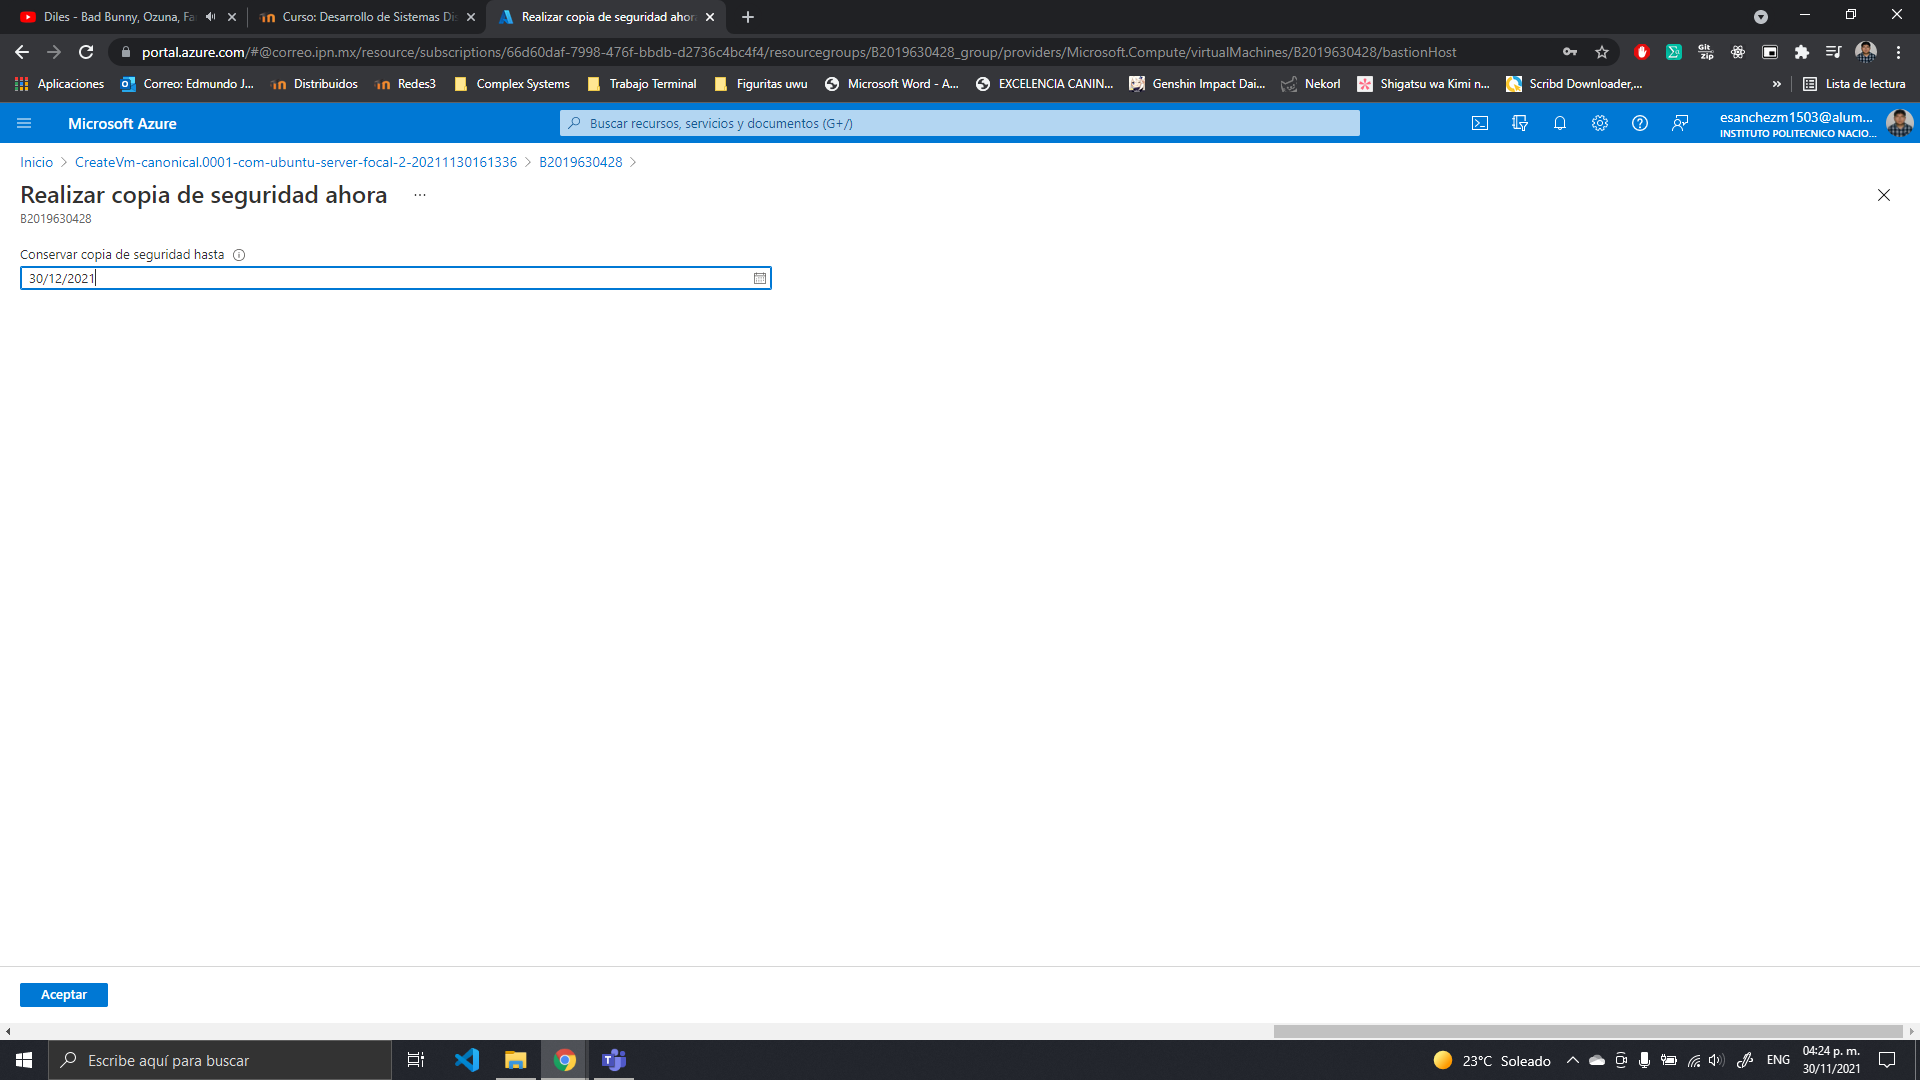
\includegraphics[scale=0.34]{resources/2.2.png}
			\caption{Creación del primer respaldo completo de la maquina virtual.}\label{fig:picture}
		\end{figure}
		 Ahora daremos clic en la campana de notificaciones para verificar que se haya iniciado el respaldo de la máquina virtual, esto lo podemos ver en la figura 11.
		 \begin{figure}[H]
			\centering
			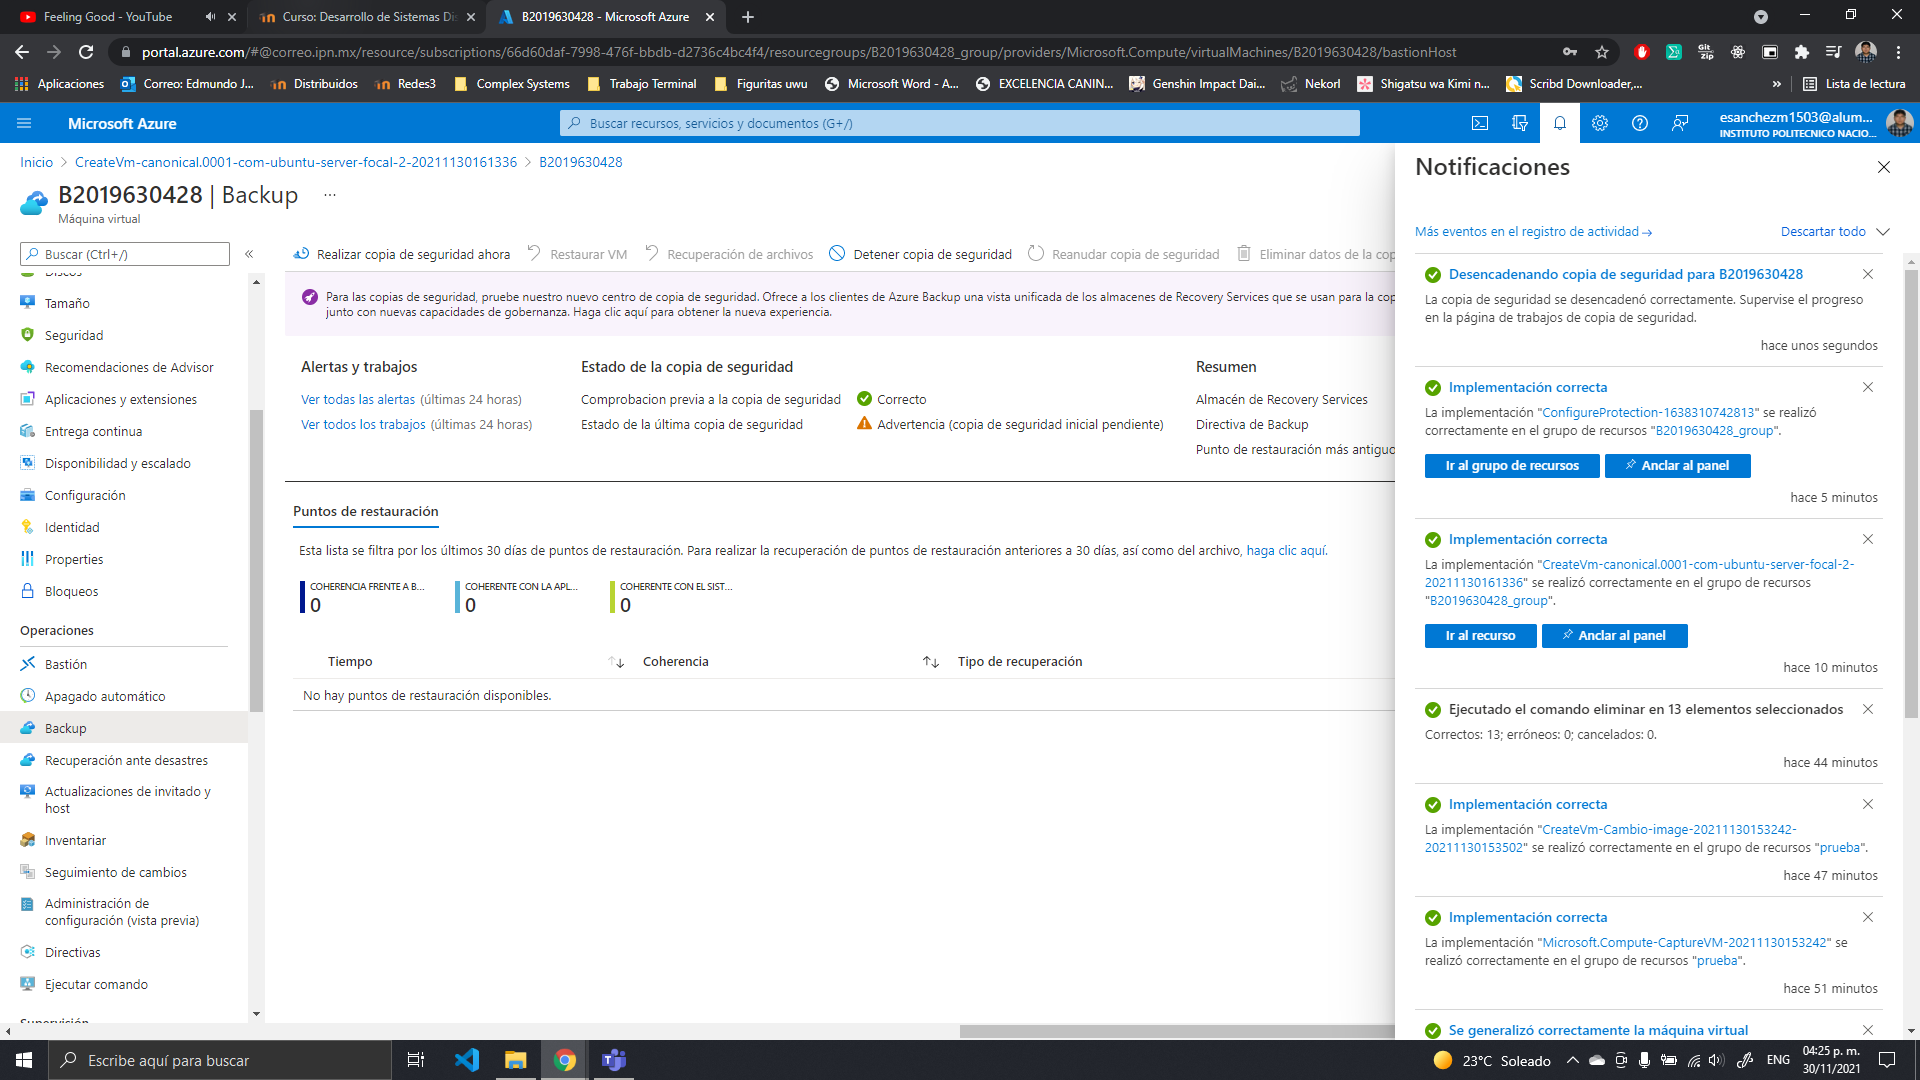
\includegraphics[scale=0.34]{resources/2.5.png}
			\caption{Inicio del primer respaldo completo de la maquina virtual.}\label{fig:picture}
		\end{figure}
		Finalmente veamos el progreso del respaldo, para ello debemos seleccionar la opción ``Ver todos los trabajos'' en la página ``Backup'' de la máquina virtual. Seleccionaremos la opción ``Actualizar'' para refrescar la pantalla que muestra el estado del proceso de respaldo, como podemos ver en la figura 12. El respaldo ha terminado cuando se despliega ``Completada'' como vemos en la figura 13. \par
		El tiempo que tarda el respaldo depende del número de procesadores virtuales, el tamaño de la memoria RAM y el tamaño del disco en la máquina virtual. El respaldo tardará más si la máquina virtual tiene poca memoria y pocos procesadores virtuales o el disco es grande, mencionar que para mi caso este proceso tomo prácticamente 1 hora para realizarse, lo cual a mi parecer es mucho, pero tomando como base lo mencionado anteriormente es normal que se haya tardado tanto ya que es la maquina con menor cantidad de recursos que se pueden crear.\par
		Una vez terminado el respaldo en la página ``Backup'' de la máquina virtual aparecerá el punto de restauración creado, como vemos en la figura 14 del siguiente paso del procedimiento.
		\begin{figure}[H]
			\centering
			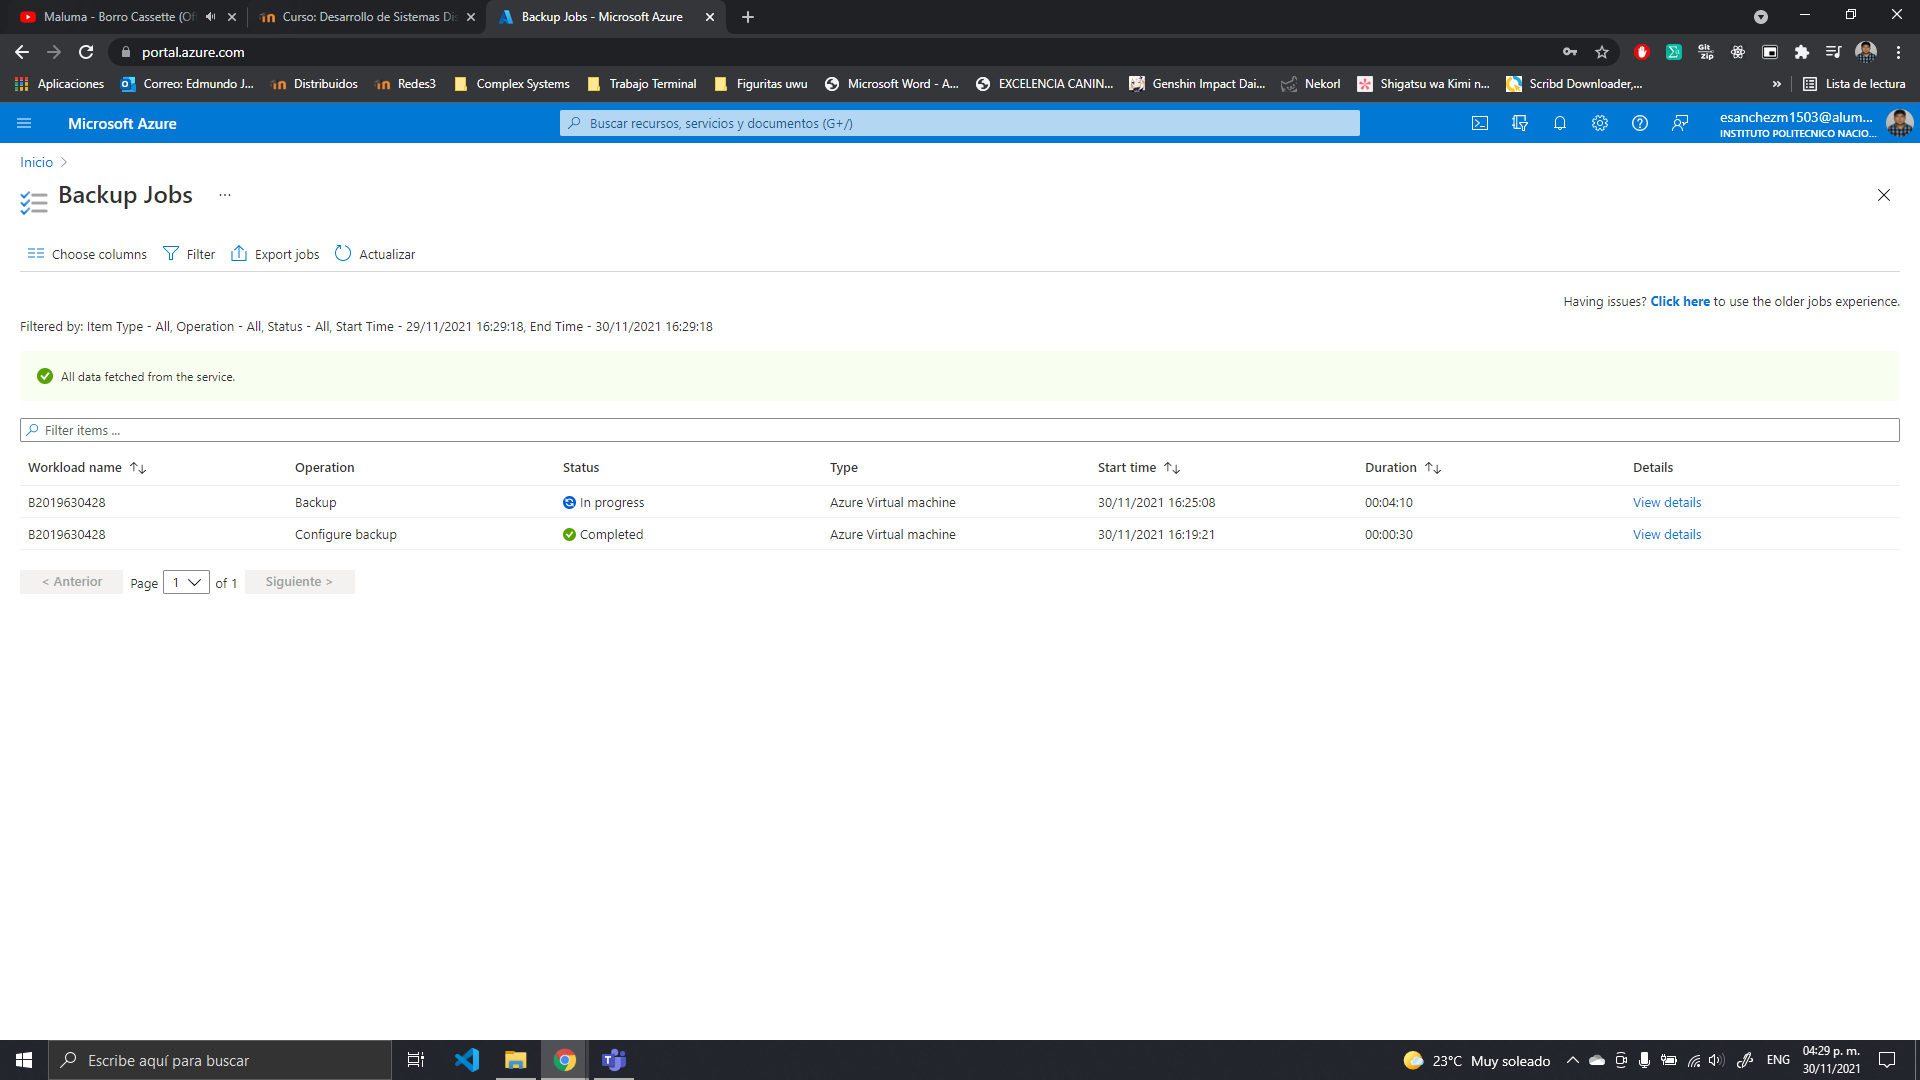
\includegraphics[scale=0.34]{resources/2.6.1.png}
			\caption{Progreso del respaldo (aun no a concluido).}\label{fig:picture}
		\end{figure}
		\begin{figure}[H]
			\centering
			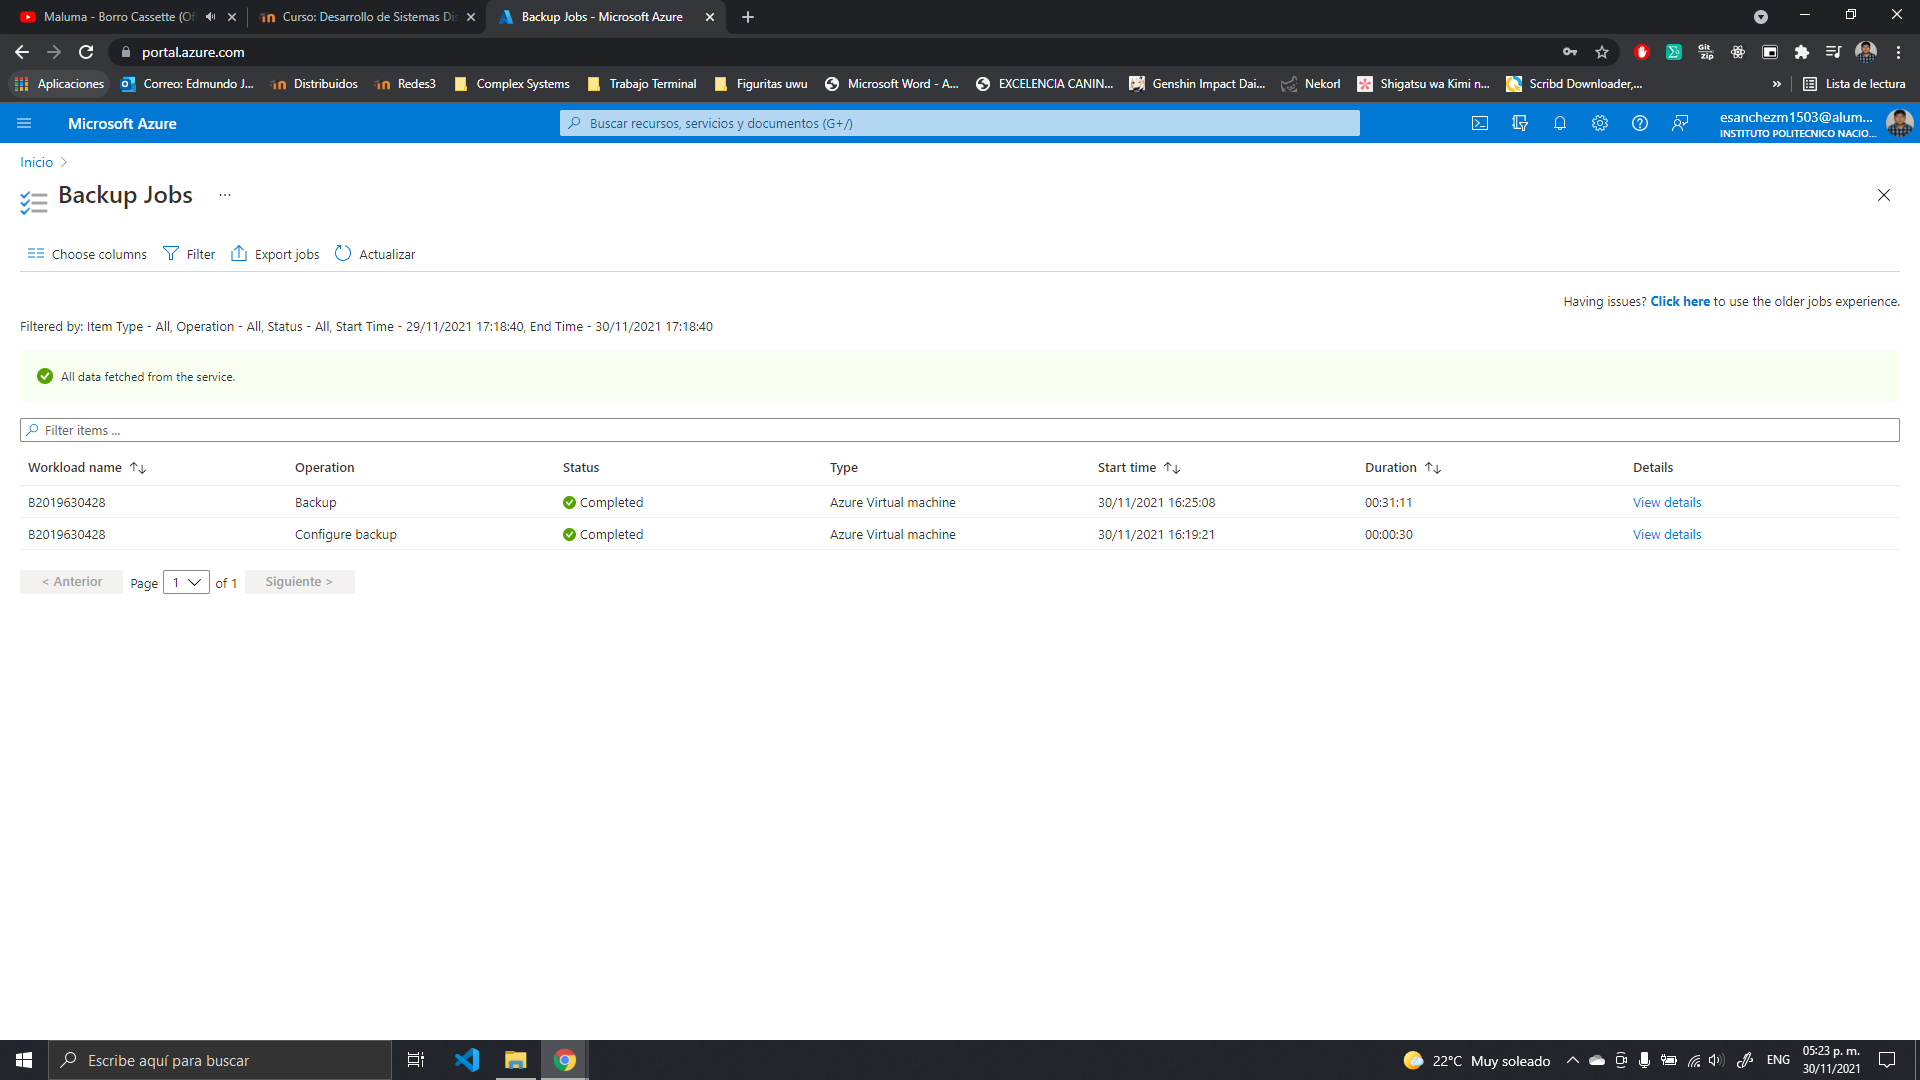
\includegraphics[scale=0.34]{resources/2.6.2.png}
			\caption{Progreso del respaldo concluido}\label{fig:picture}
		\end{figure}
		\subsection{Restaurar la máquina virtual}
		Ahora volvemos a ir a nuestra maquina virtual al apartado de ``Backup'' y damos clic a la opción de ``Restaurar VM'', como vemos en la figura 14.
		\begin{figure}[H]
			\centering
			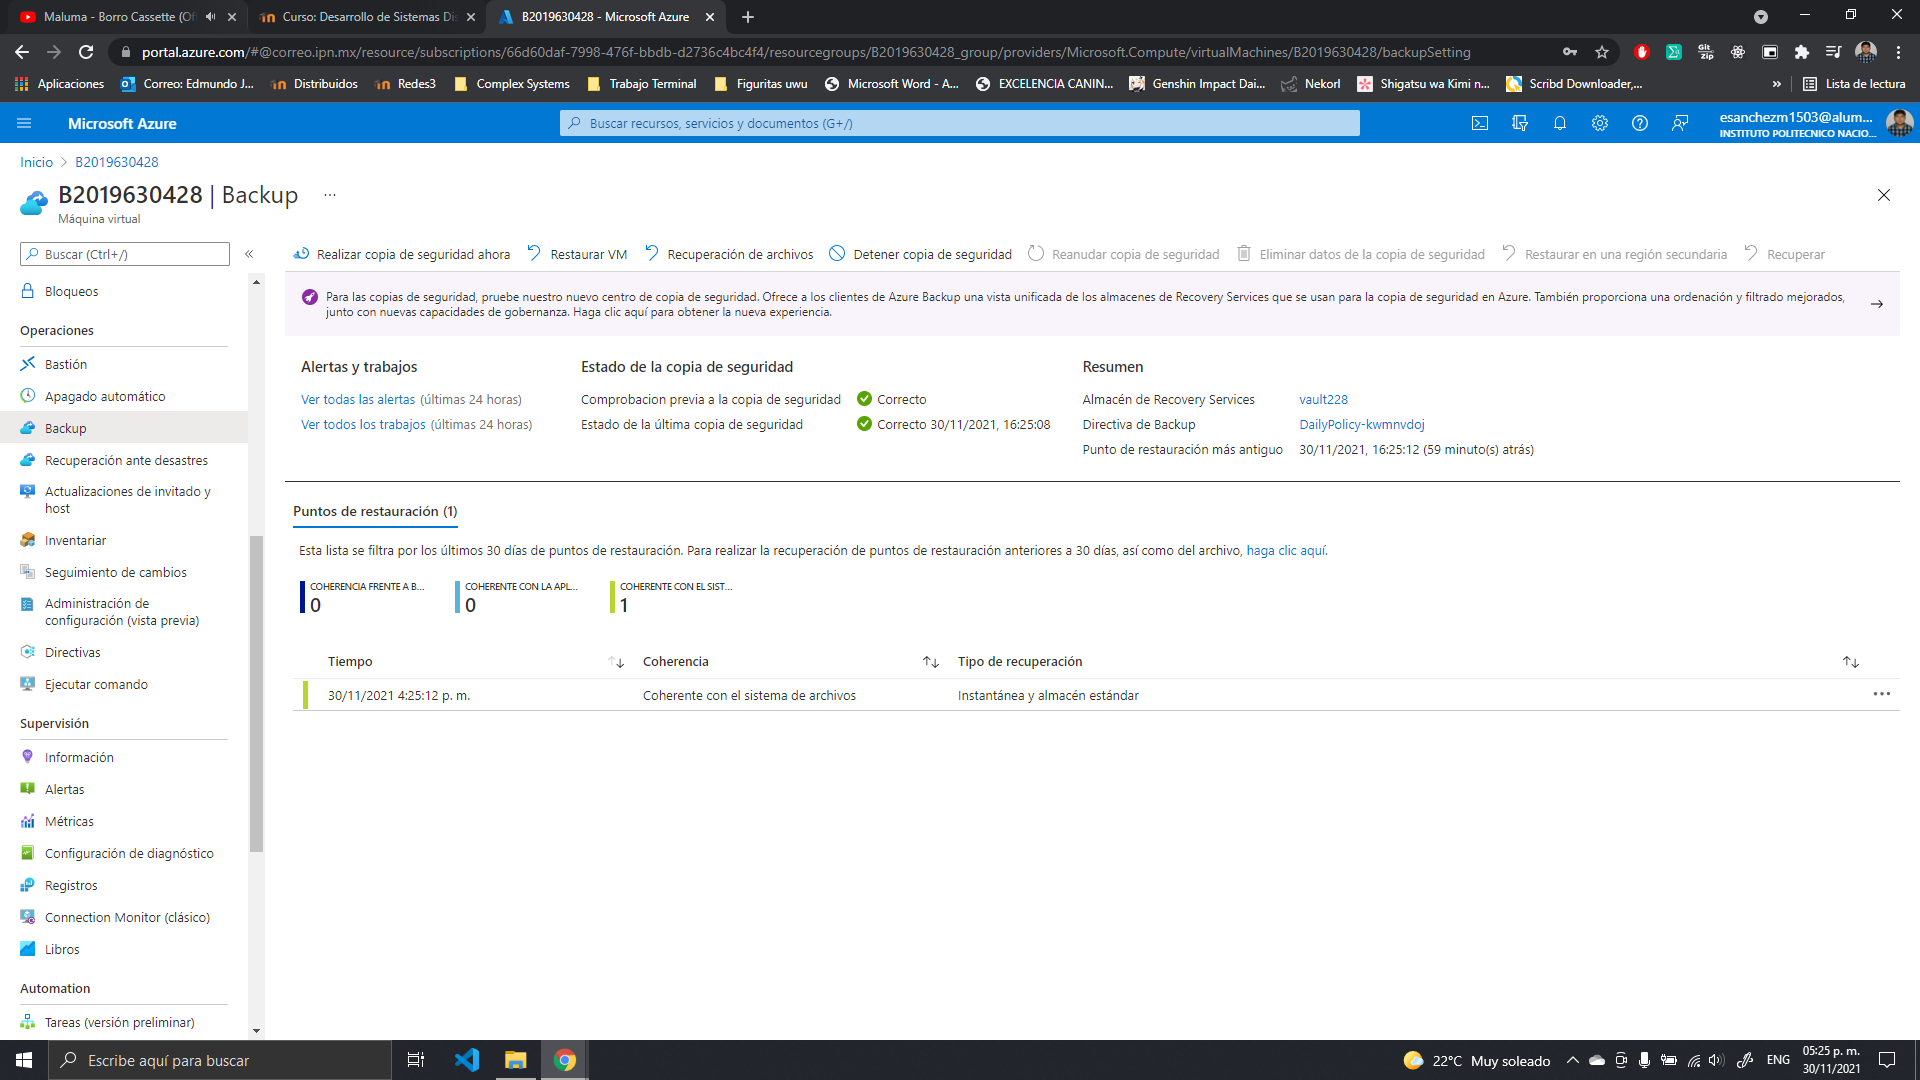
\includegraphics[scale=0.34]{resources/3.1-2.png}
			\caption{Opción ``Backup'' dentro de la maquina virtual.}\label{fig:picture}
		\end{figure}
		Luego en ``Punto de restauración'' damos clic en la opción ``Seleccionar'', para posteriormente seleccionar el punto de restauración (panel derecho) y damos clic en el botón ``Aceptar'', como vemos en la figura 15.
		\begin{figure}[H]
			\centering
			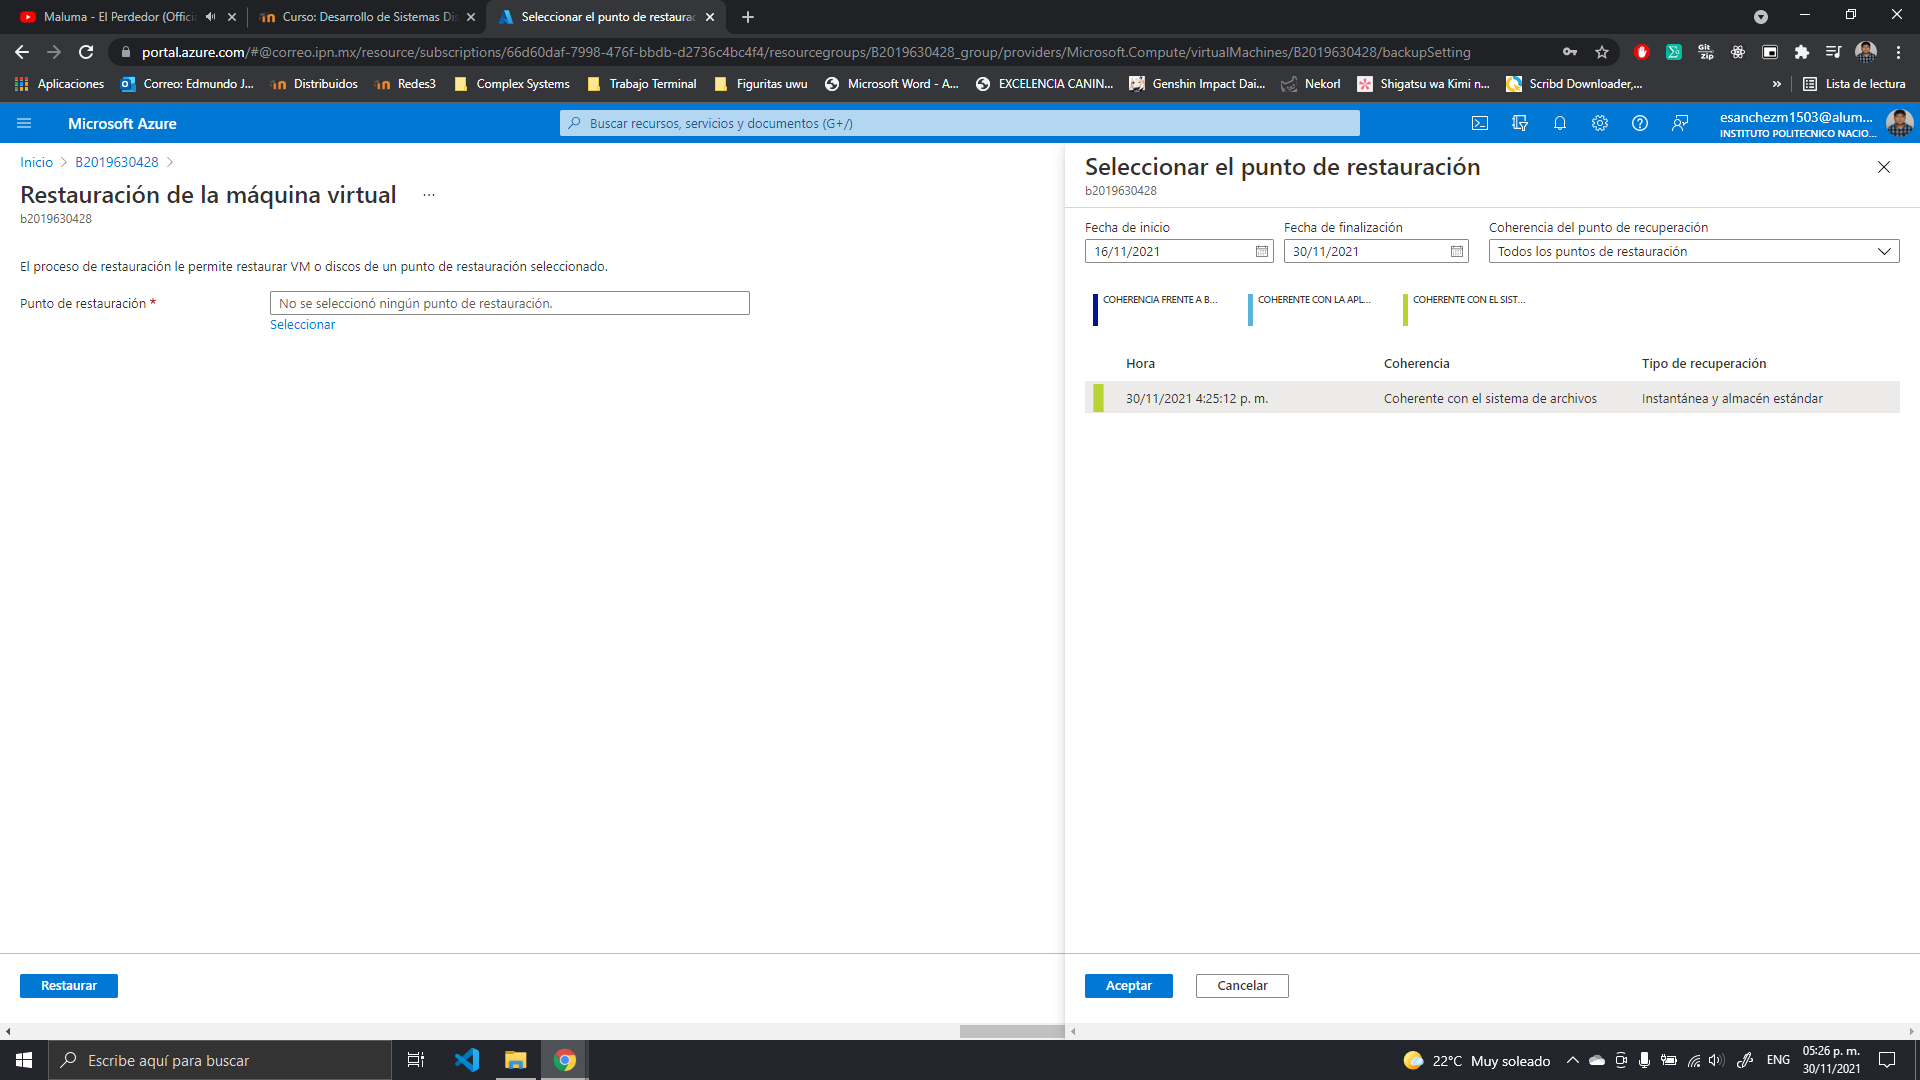
\includegraphics[scale=0.34]{resources/3.3-4.png}
			\caption{Seleccionando punto de restauración.}\label{fig:picture}
		\end{figure}
		 En ``Tipo de restauración'' seleccionamos ``Crear una nueva máquina virtual'',ingresamos el nombre de la nueva máquina virtual, seleccionamos la misma red virtual que la maquina que creamos para la practica y finalmente seleccionamos la ubicación del almacenamiento provisional, esta cuenta de almacenamiento se utilizará temporalmente durante la restauración, todo esto lo podremos ver en la figura 16 notar que ya tenemos seleccionado una cuenta de almacenamiento que se creo para esta practica, el procedimiento para la creación de la cuenta de almacenamiento lo podemos ver en la sección 2.4.1.
		 \begin{figure}[H]
			\centering
			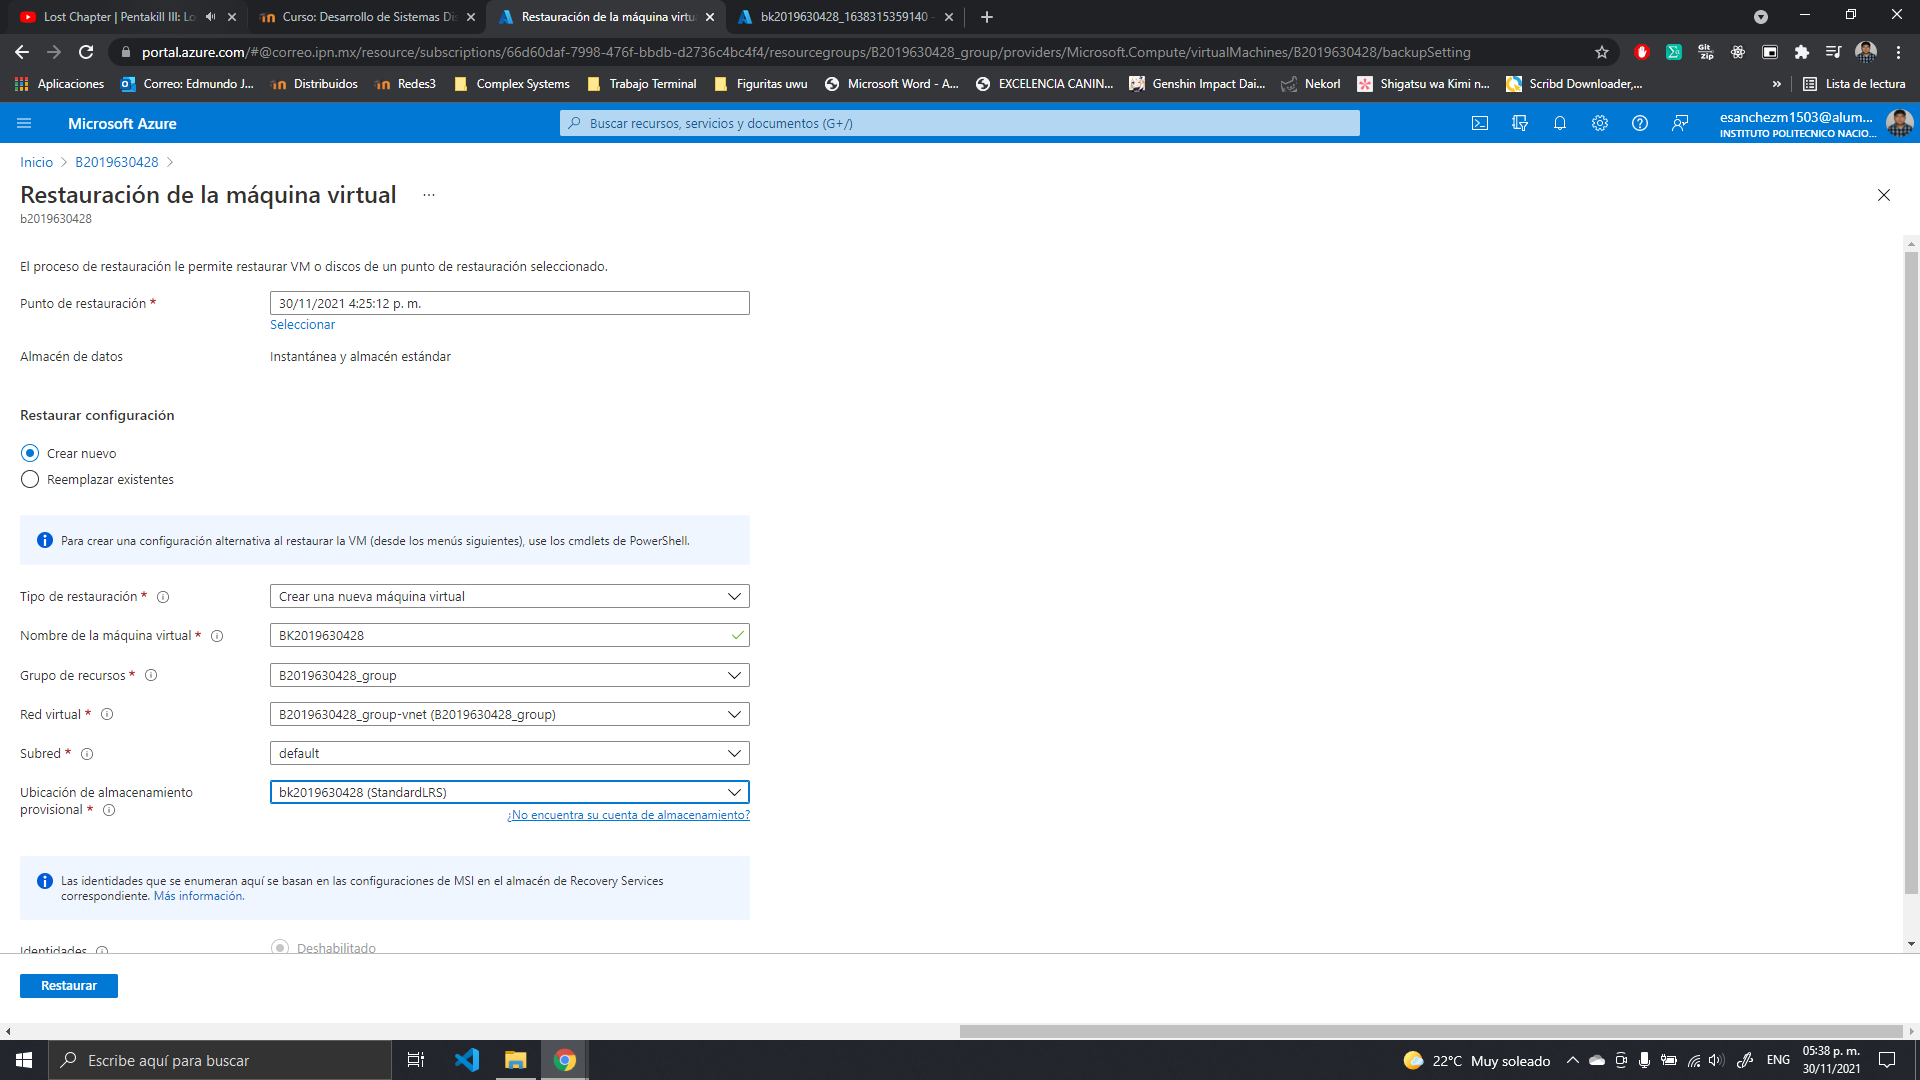
\includegraphics[scale=0.34]{resources/3.6-9.png}
			\caption{Restauración de una maquina virtual.}\label{fig:picture}
		\end{figure}
			\subsubsection{Creación de la cuenta de almacenamiento }
			Nos dirigimos a la ventana de búsqueda de Azure ahí escribimos: cuentas de almacenamiento e ingresamos a la primera opción mostrada como podemos ver en la figura 17.
				\begin{figure}[H]
					\centering
					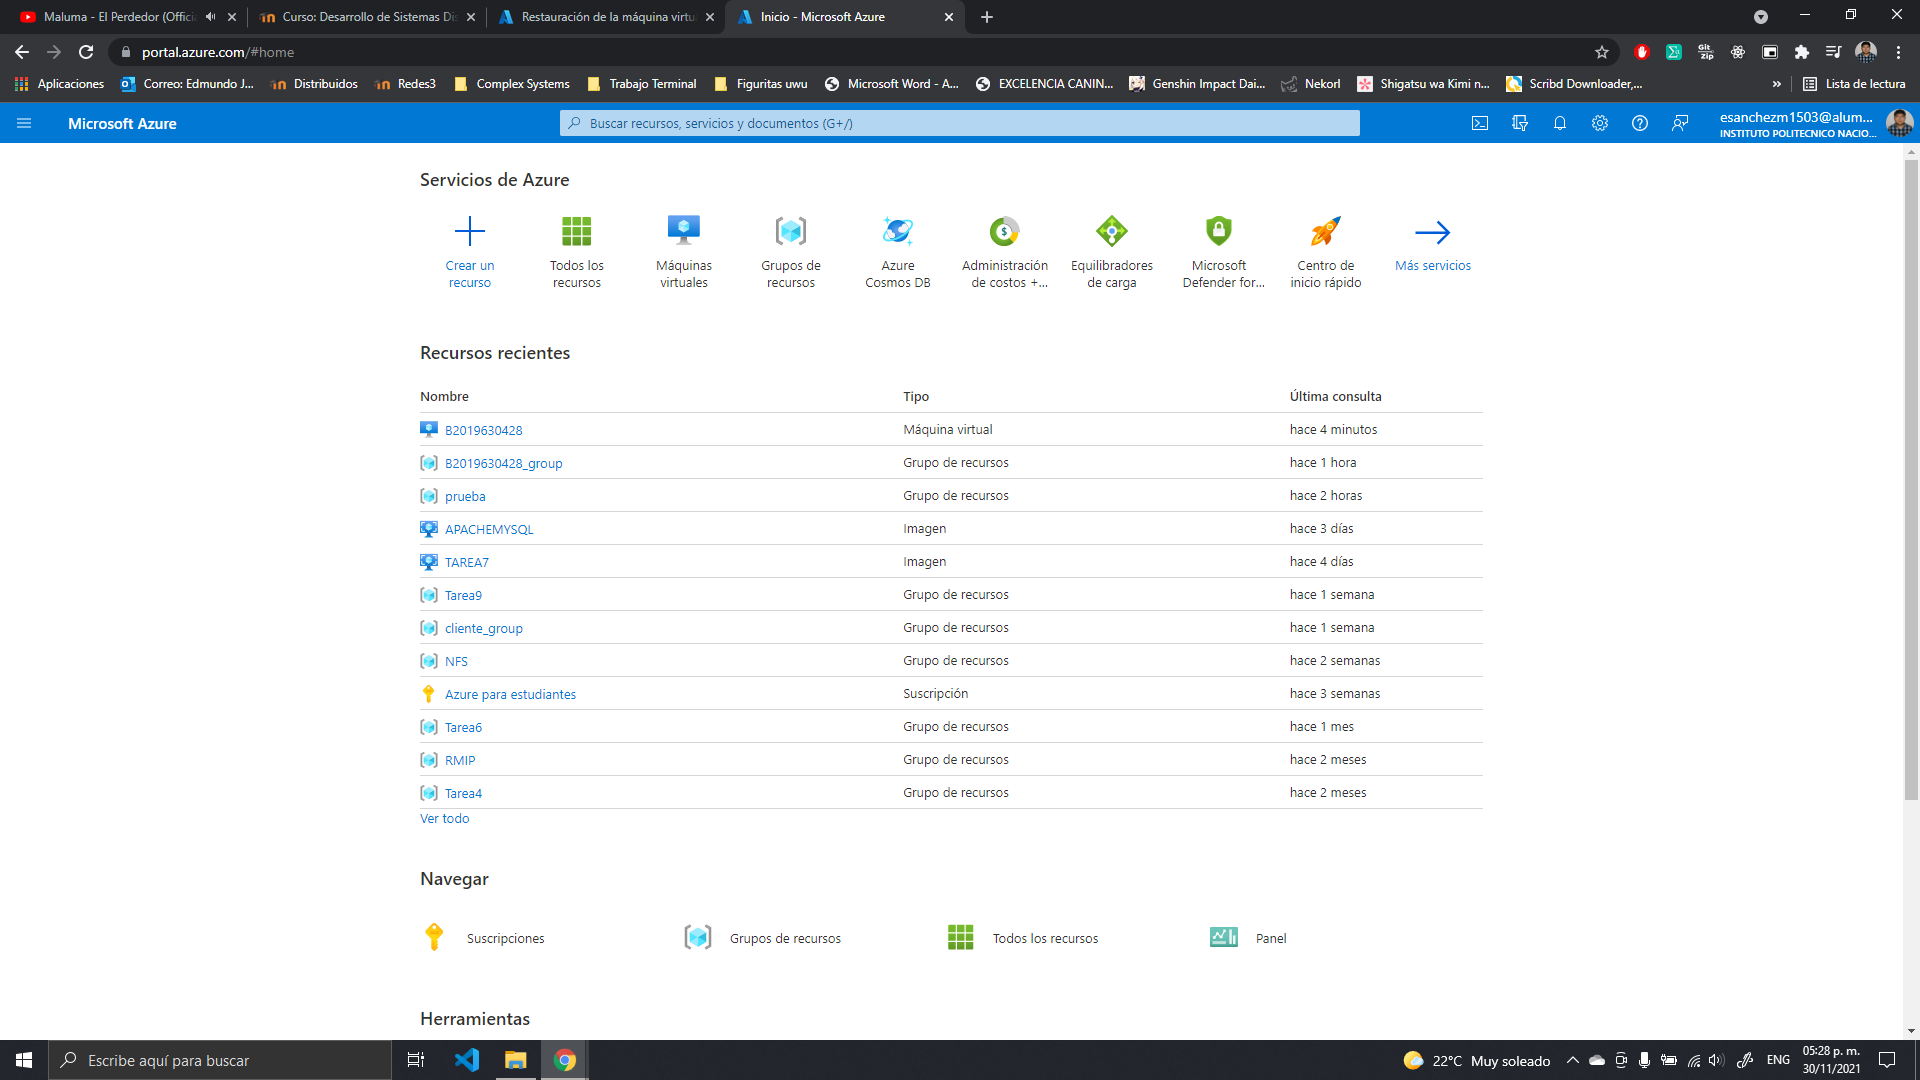
\includegraphics[scale=0.34]{resources/almacenamiento0.png}
					\caption{Portal de Azure.}\label{fig:picture}
				\end{figure}
			Ahora como vemos en la figura 18 damos clic en la opcion +Crear.
				\begin{figure}[H]
					\centering
					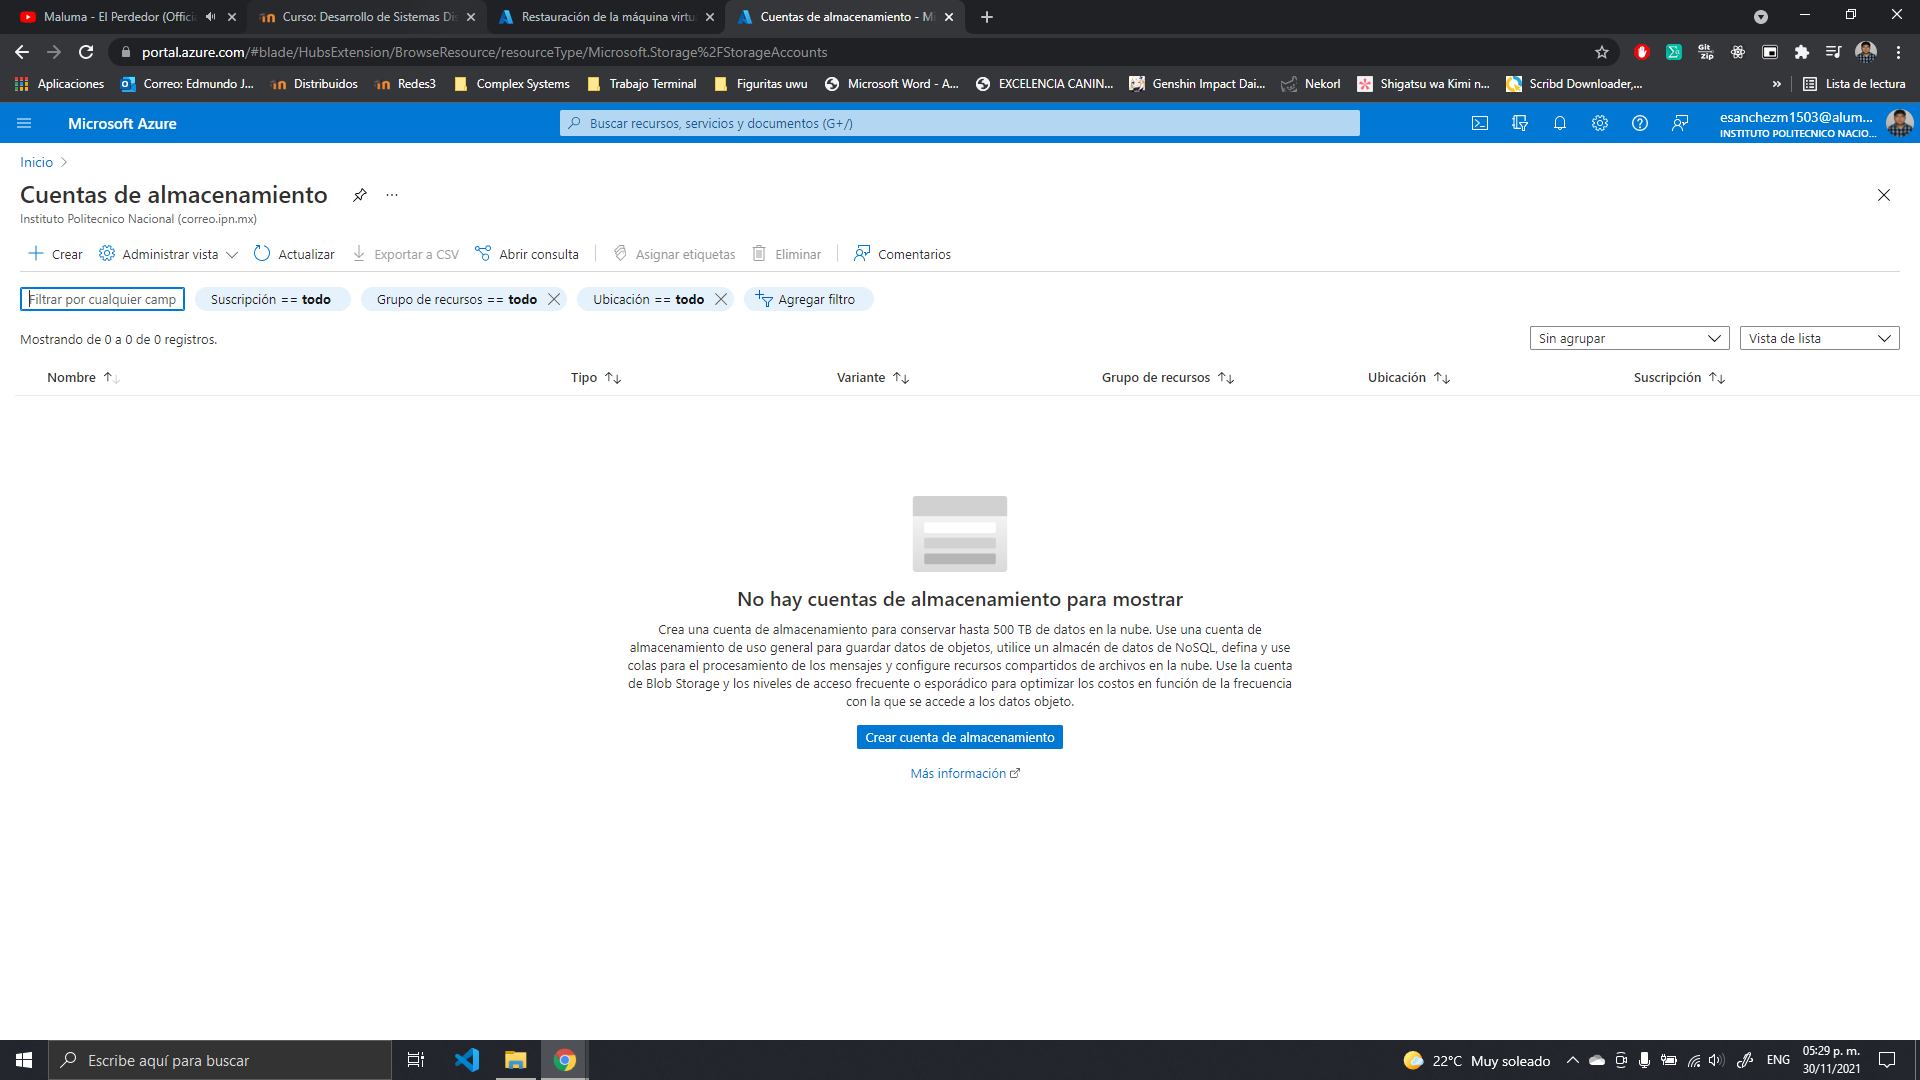
\includegraphics[scale=0.34]{resources/almacenamiento1.png}
					\caption{Cuentas de almacenamiento.}\label{fig:picture}
				\end{figure}
			Ahora solo rellenamos los datos solicitados, seleccionamos el grupo de recursos de la máquina virtual que se creo al inicio, ingresamos un nombre para la cuenta de almacenamiento (no debe existir en Azure), seleccionamos la misma ubicación del vault (almacén de Recovery Services) en el procedimiento (en este caso Este de EE.UU.), habilitamos el respaldo de una máquina virtual en Azure y finalmente en ``Replicación'' seleccionamos ``Almacenamiento con redundancia local (LRS)'', todo esto lo podemos ver la figura 19.
				\begin{figure}[H]
					\centering
					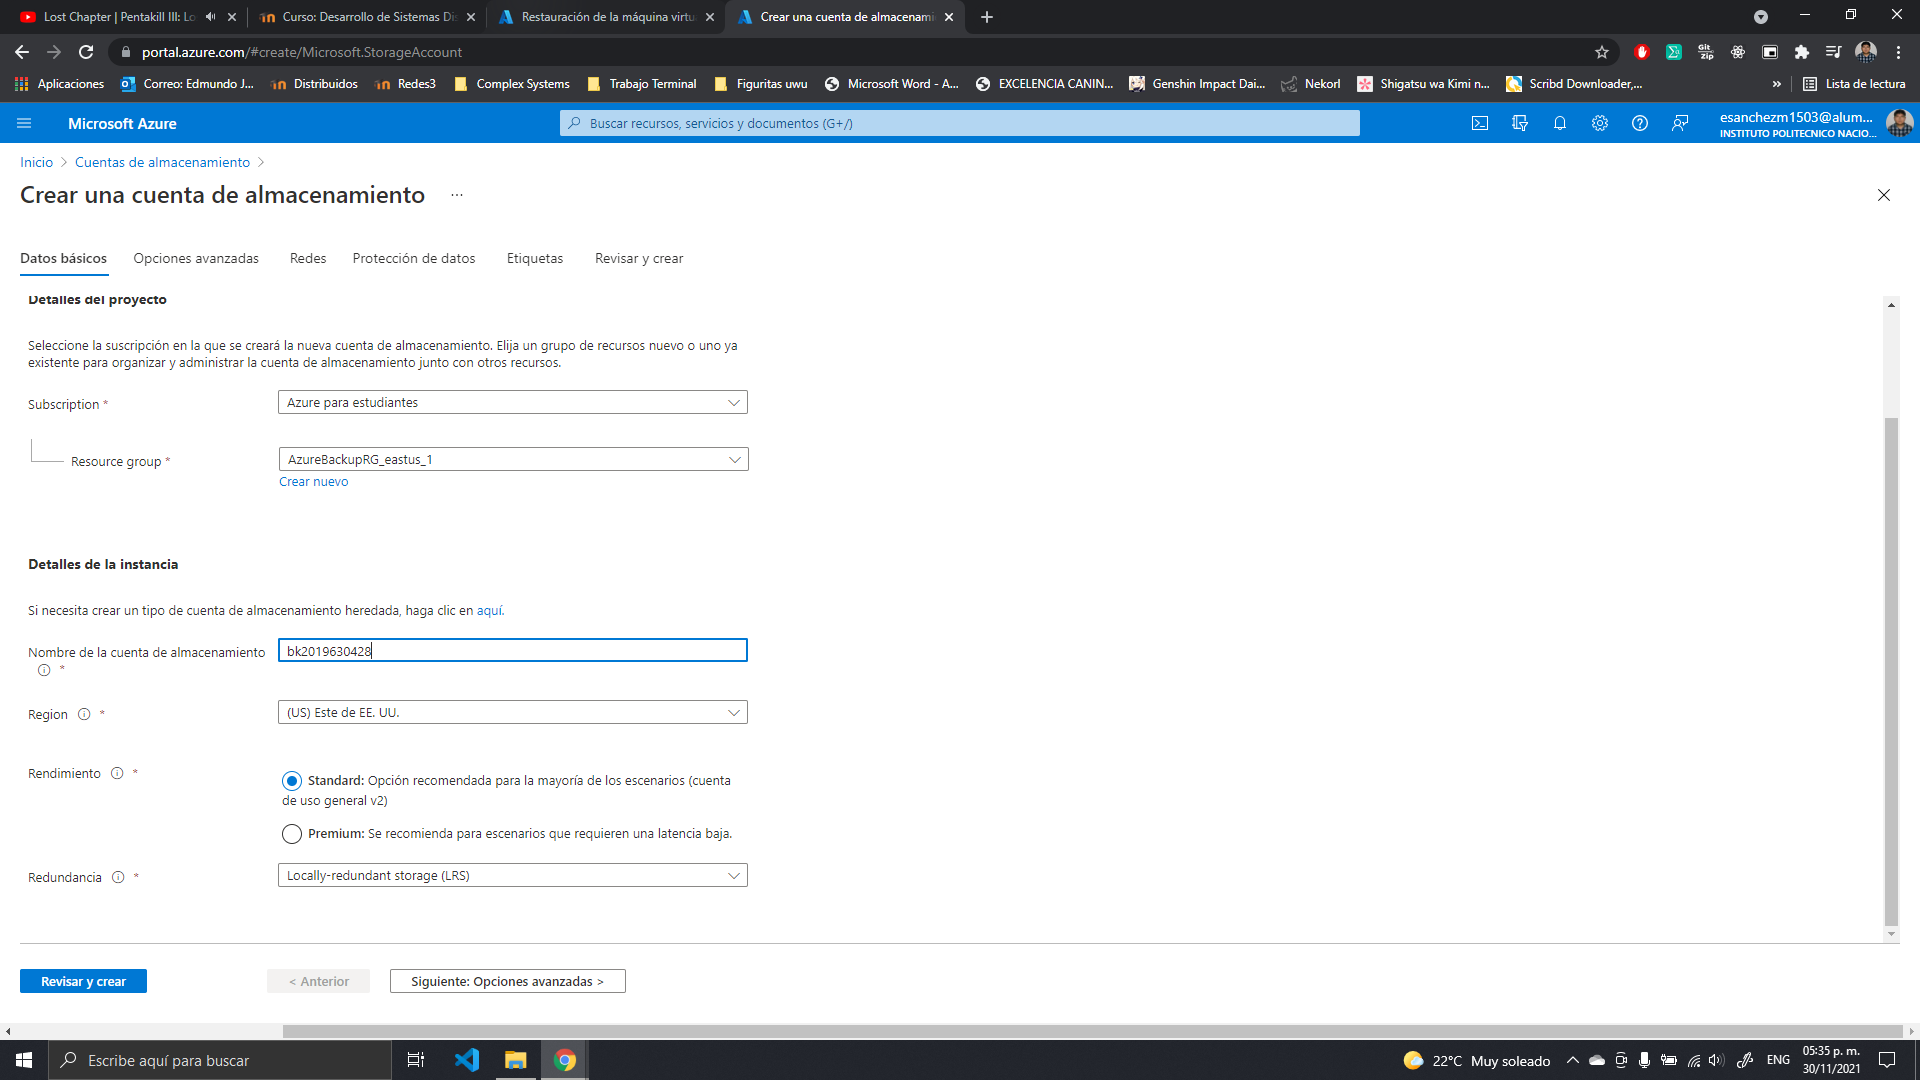
\includegraphics[scale=0.34]{resources/almacenamiento2.png}
					\caption{Datos básicos de la cuenta de almacenamiento.}\label{fig:picture}
				\end{figure}
			Finalmente vamos a la opción de ``Revisar y crear'' y finalmente damos clic al botón de ``Crear'' esto lo podemos ver la figura 20 y en la figura 21 vemos como se creo de manera exitosa.
				\begin{figure}[H]
					\centering
					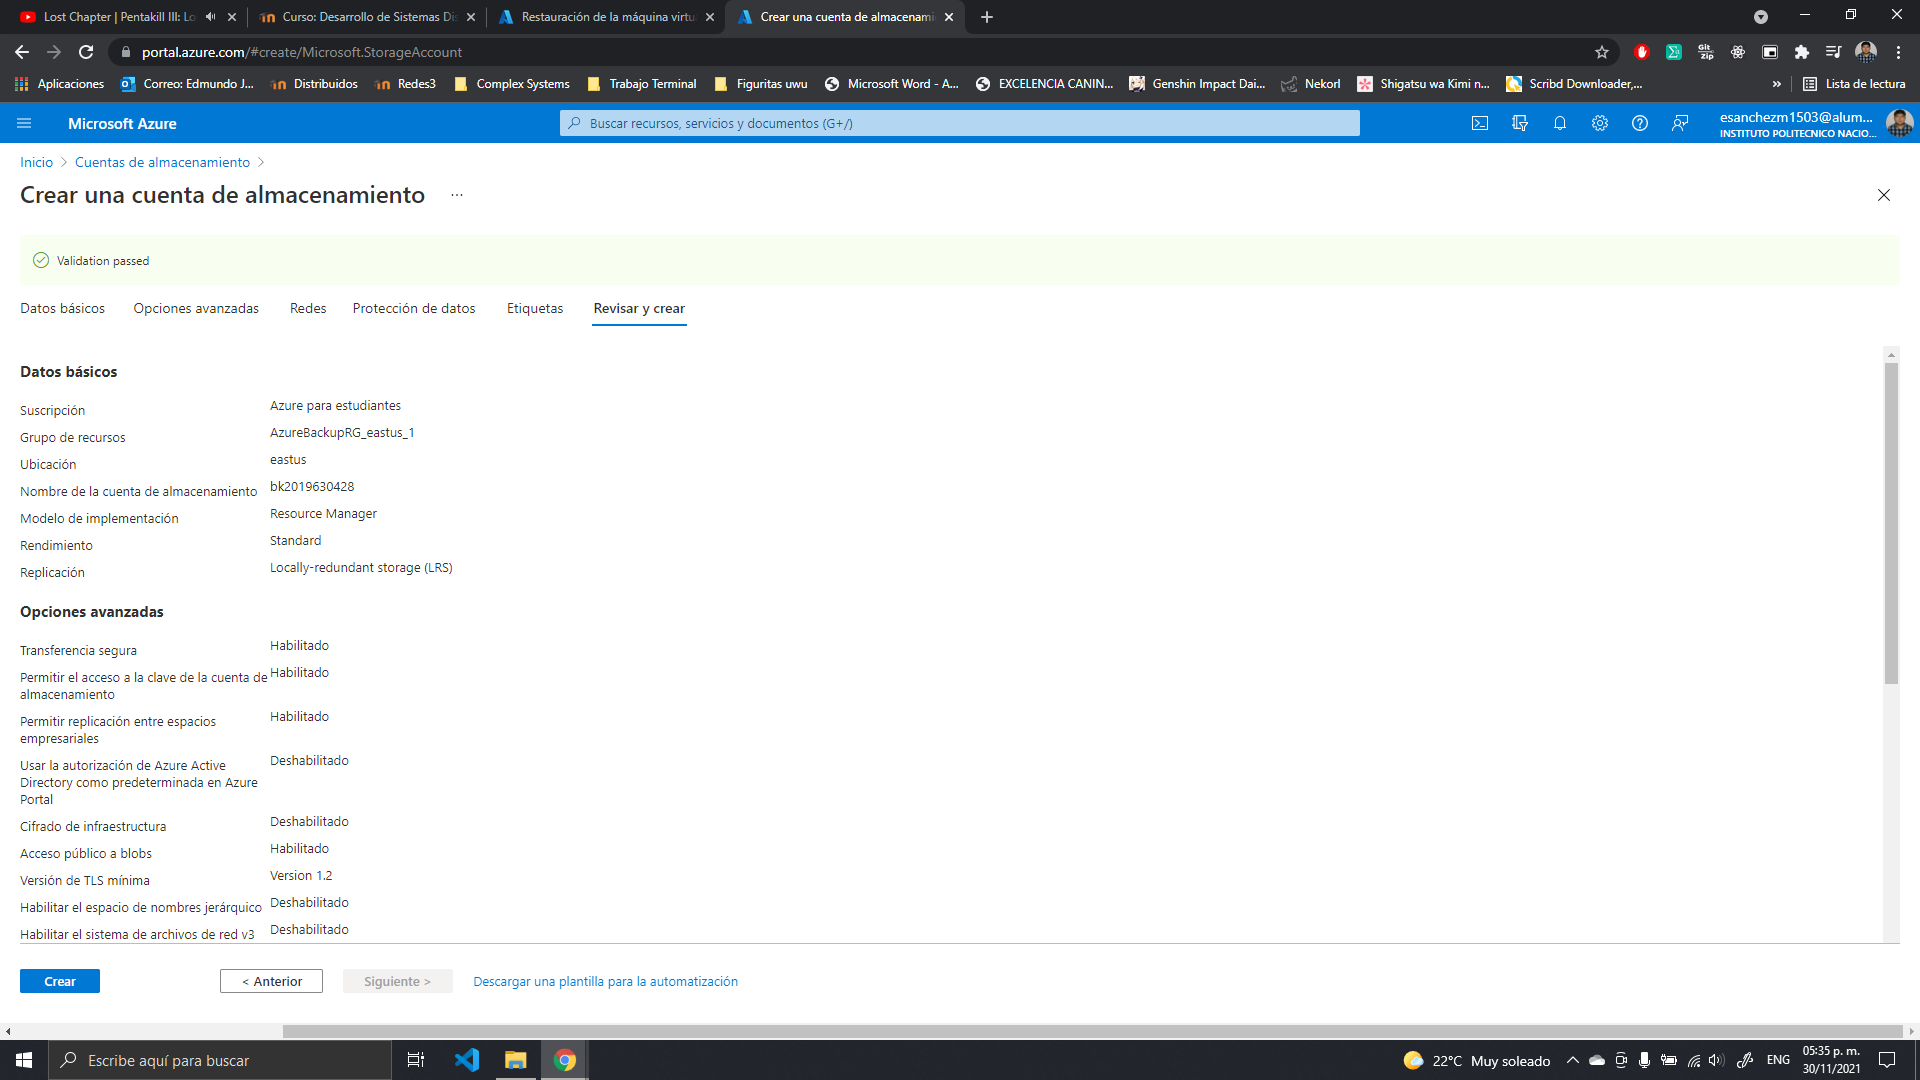
\includegraphics[scale=0.34]{resources/almacenamiento3.png}
					\caption{Revisar y crear la cuenta de almacenamiento.}\label{fig:picture}
				\end{figure}
				\begin{figure}[H]
					\centering
					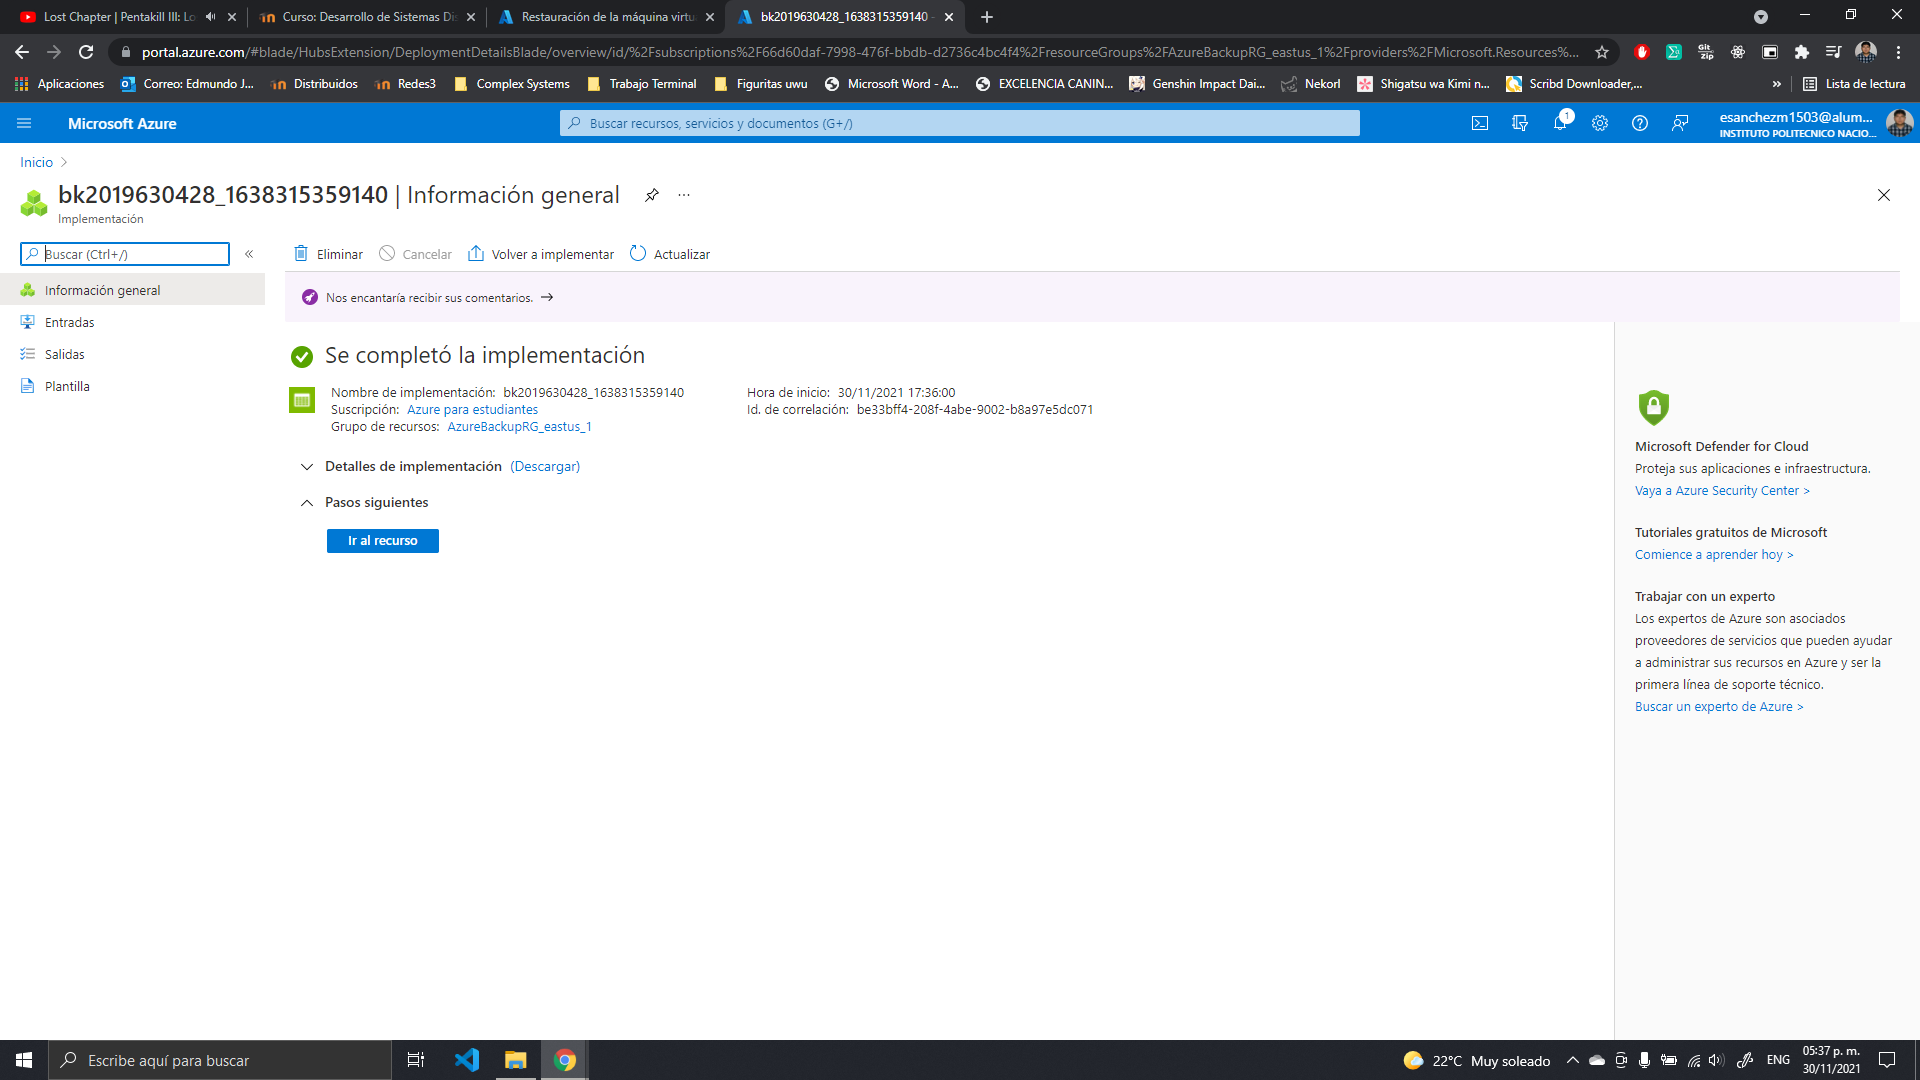
\includegraphics[scale=0.34]{resources/almacenamientoF.png}
					\caption{Cuenta de almacenamiento creada de manera exitosa.}\label{fig:picture}
				\end{figure}
		\subsection*{}
    		Ahora damos clic en el botón ``Restaurar'' y nos dirigimos a ``Ver todos los trabajos'' en la página ``Backup'' de la máquina virtual para ver el progreso de la restauración seleccionar la opción, esto lo podemos ver en la figura 22. Seleccionamos la opción ``Actualizar'' para refrescar la pantalla que muestra el estado del proceso de restauración, esto lo podemos ver en la figura 23, cabe mencionar que este proceso tomo muy poco tiempo a diferencia del proceso de respaldo, solo tomo 4 minutos.
		\begin{figure}[H]
			\centering
			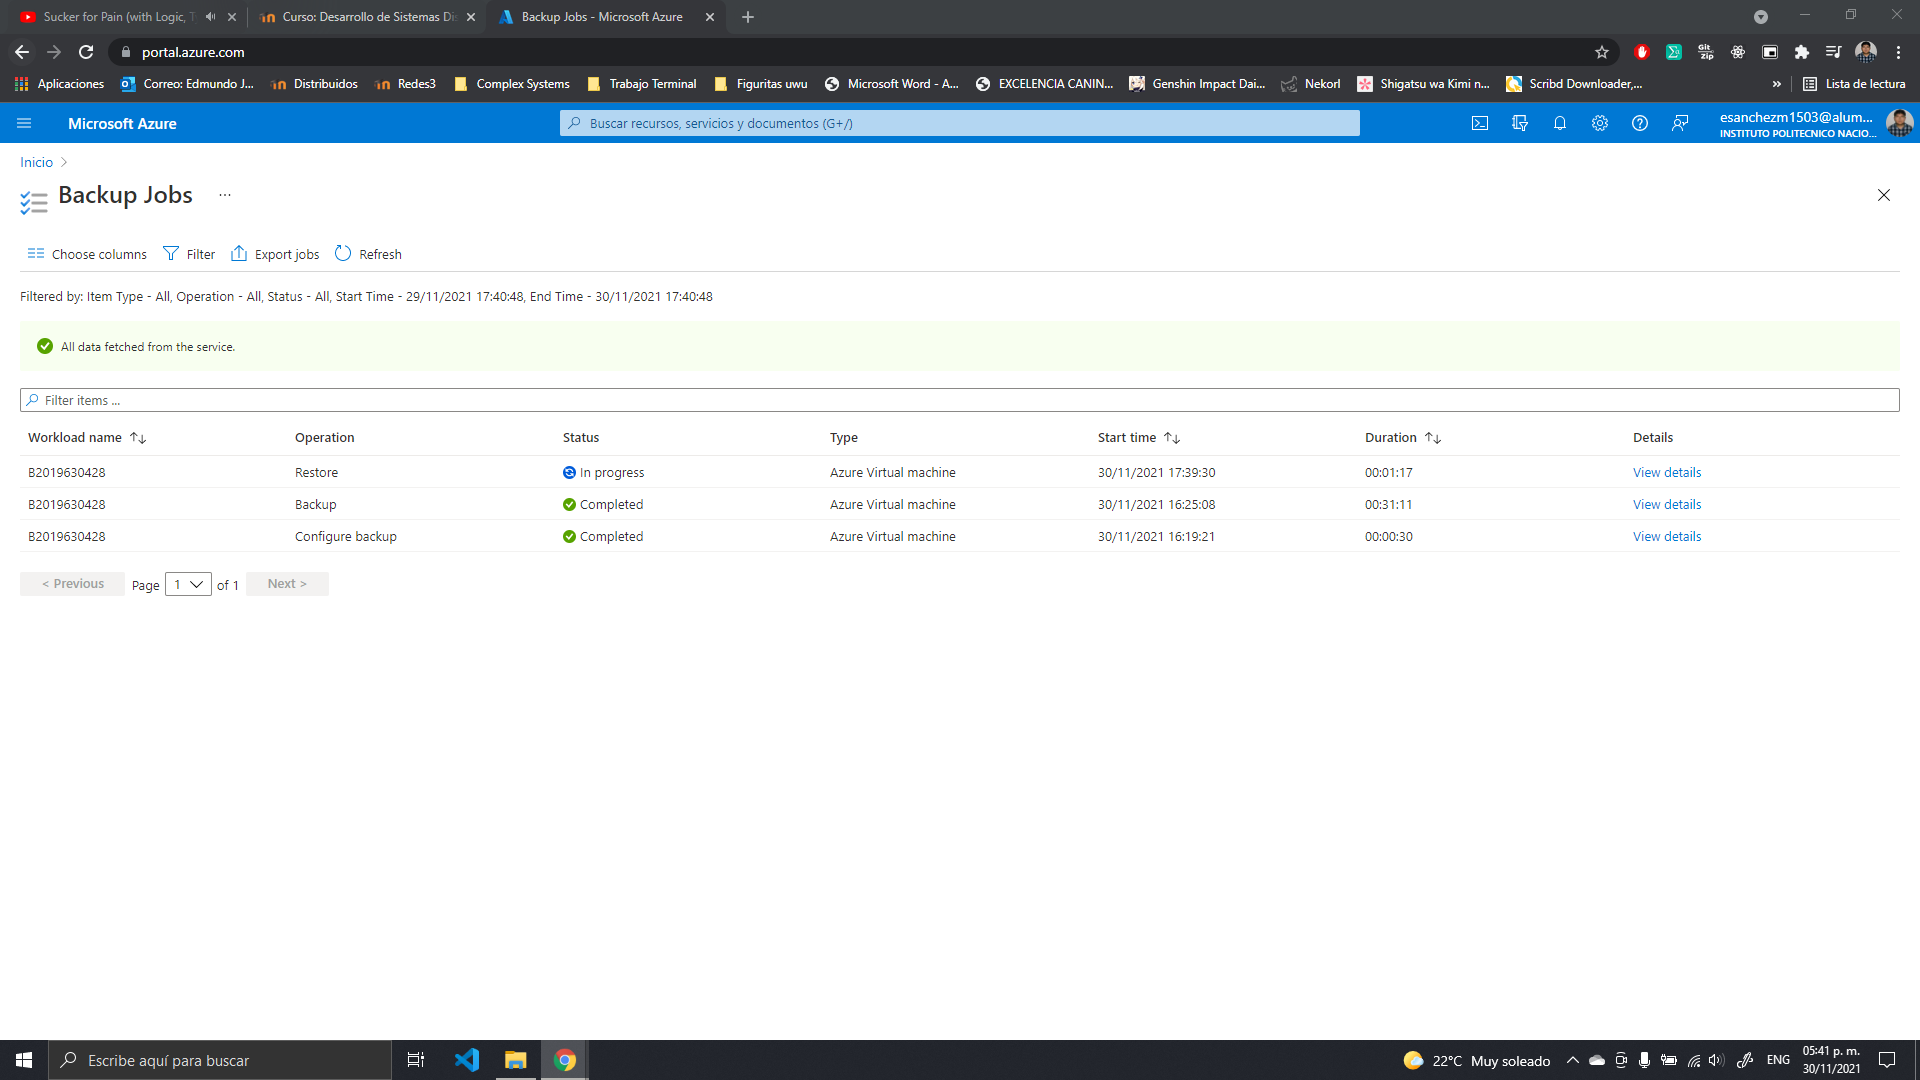
\includegraphics[scale=0.34]{resources/3.11.png}
			\caption{Restauración de una maquina virtual en proceso.}\label{fig:picture}
		\end{figure}
		\begin{figure}[H]
			\centering
			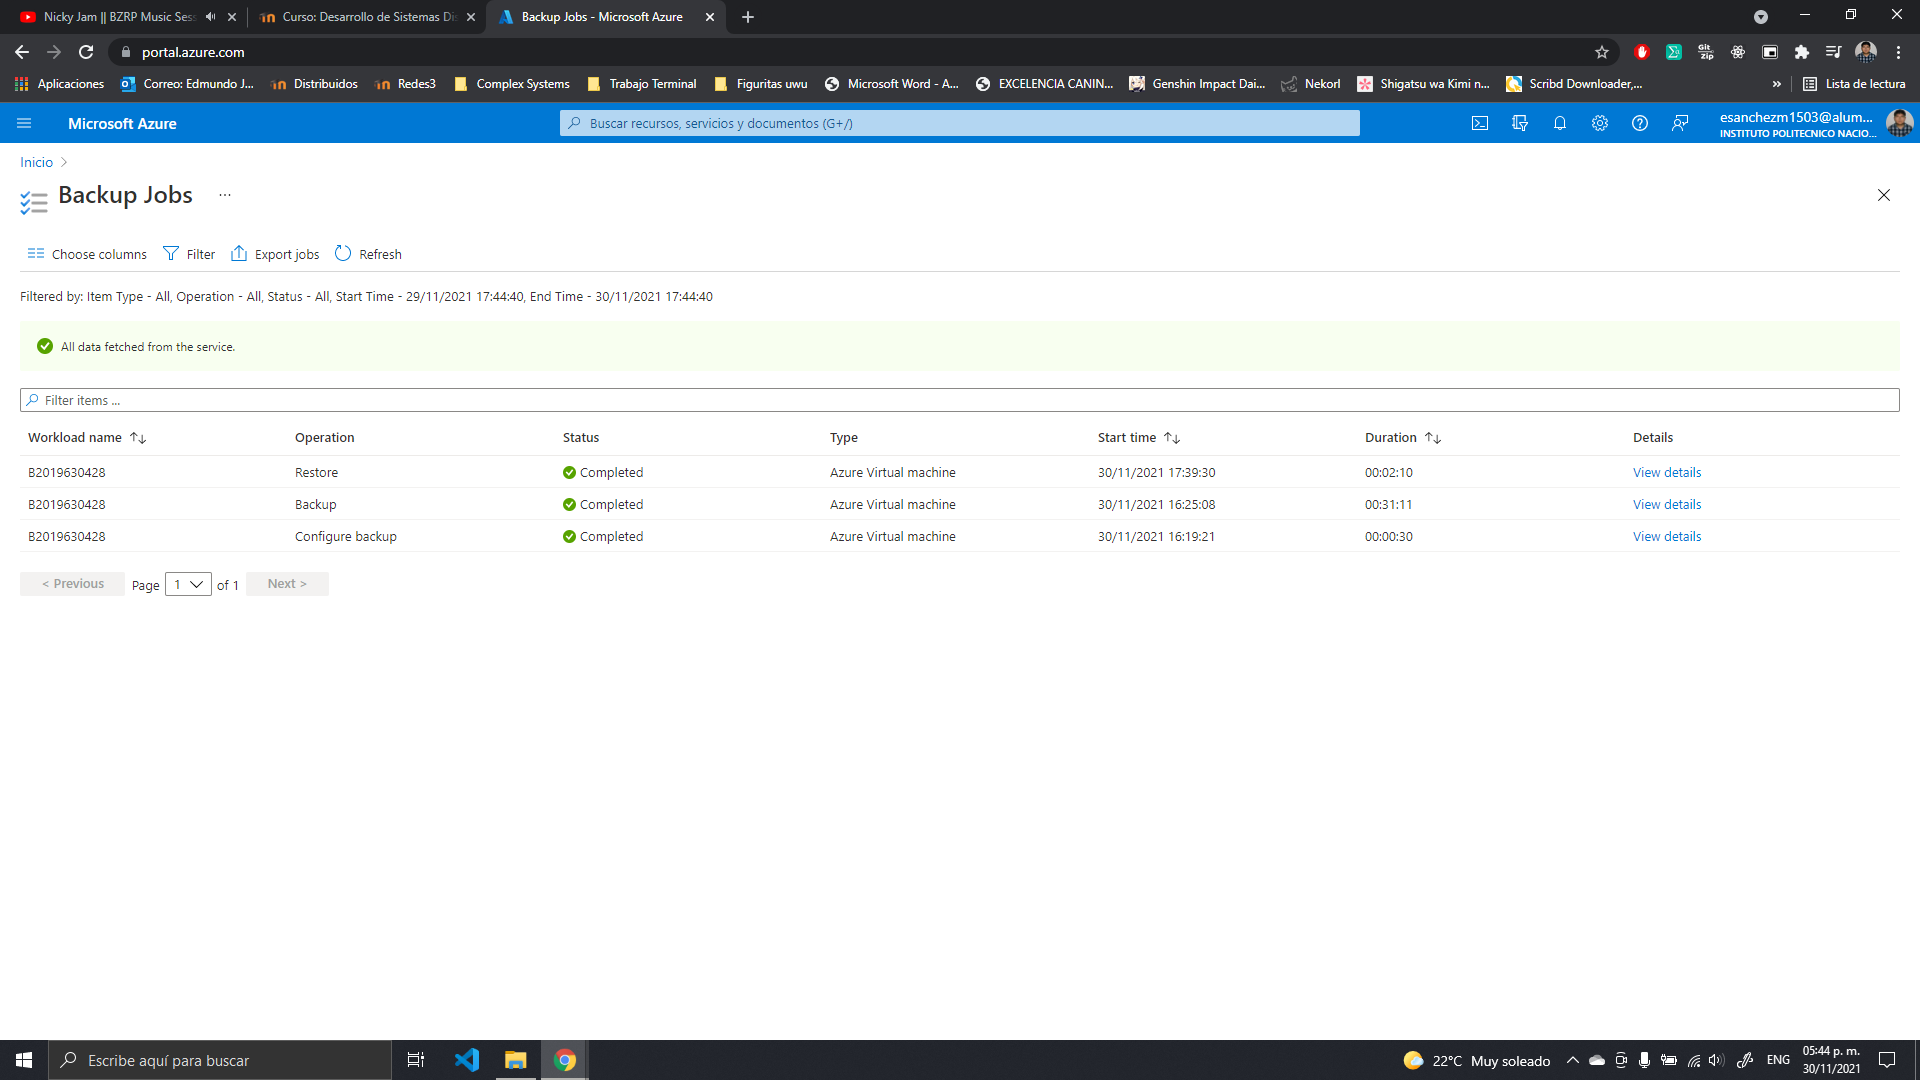
\includegraphics[scale=0.34]{resources/3.12.png}
			\caption{Restauración de una maquina virtual finalizado.}\label{fig:picture}
		\end{figure}
			Una vez finalizado la restauración de la maquina virtual podemos ir al portal de Azure para poder ver la lista de maquinas virtuales existentes que en ese momento estaban disponibles, esto lo vemos en la figura 24.
		\begin{figure}[H]
			\centering
			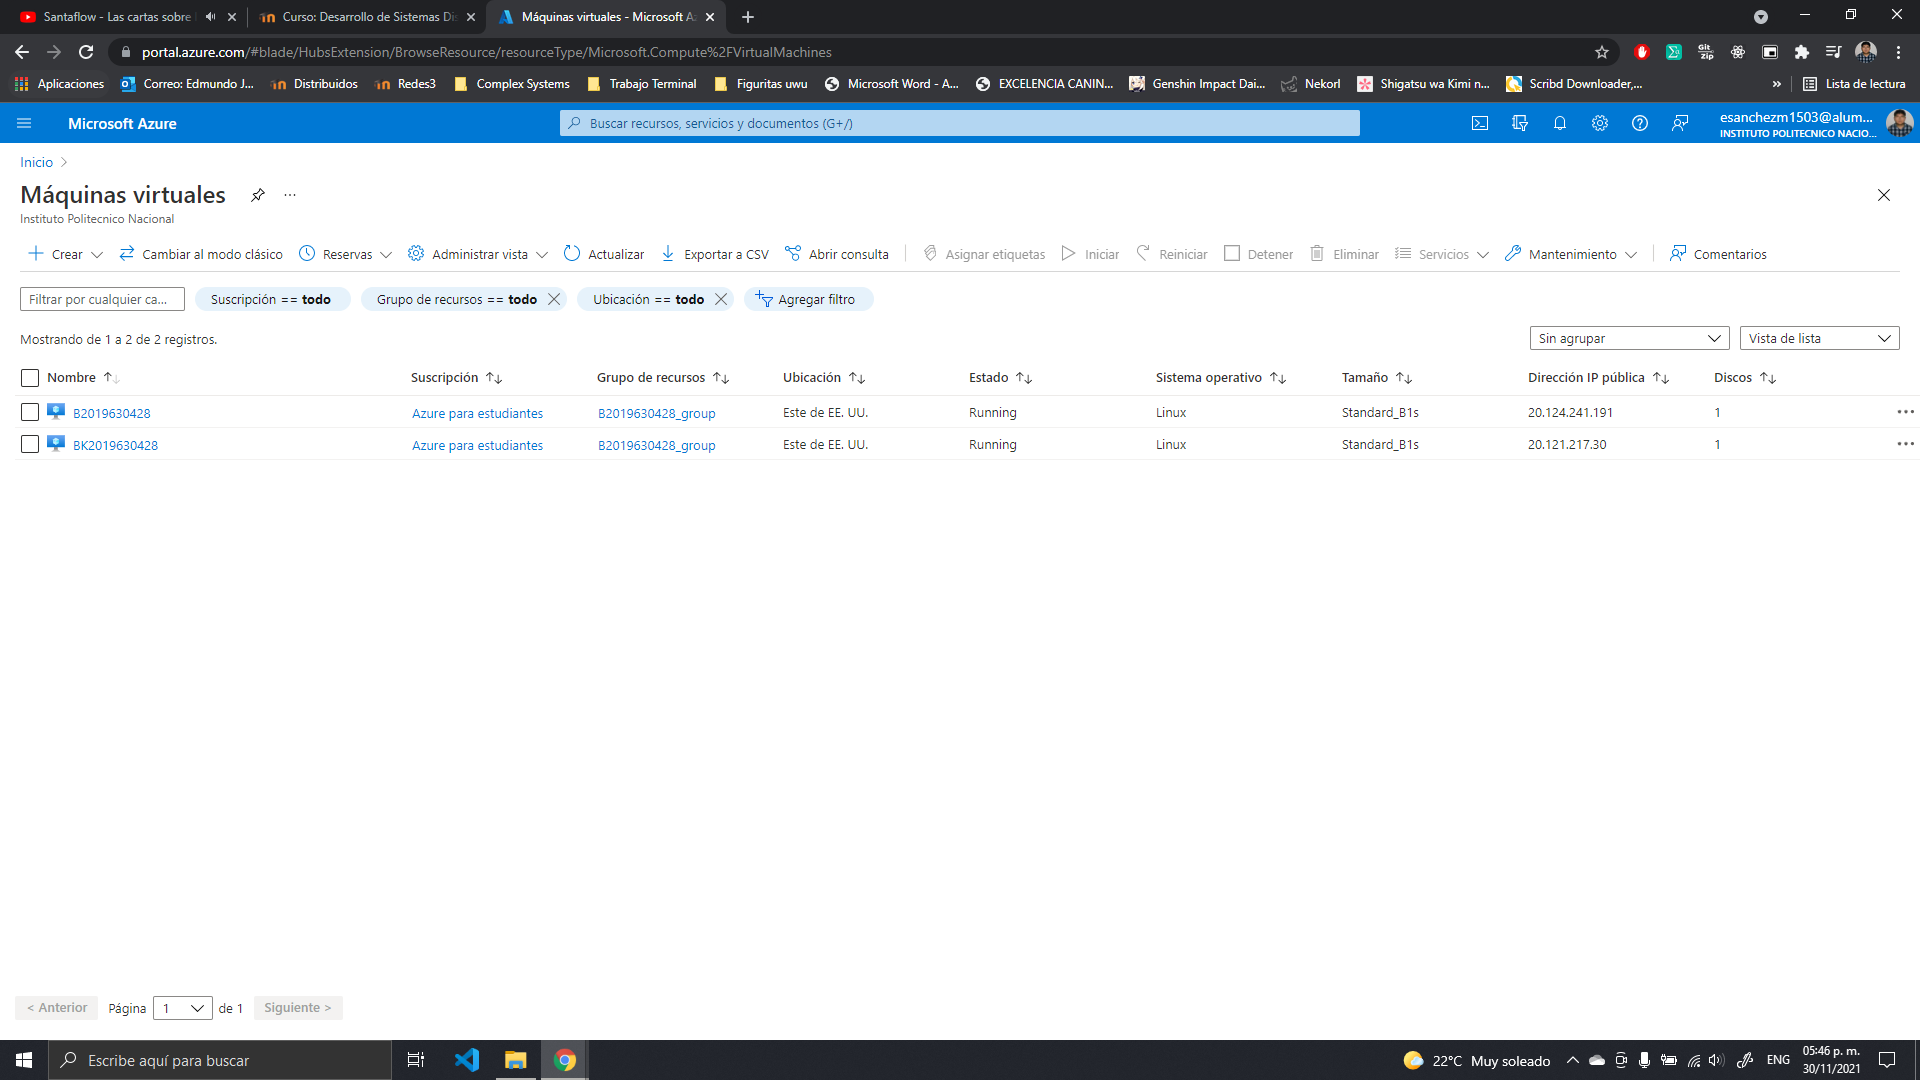
\includegraphics[scale=0.34]{resources/3.13.png}
			\caption{Maquinas virtuales existentes en Azure.}\label{fig:picture}
		\end{figure}
		También podemos ver como a pesar de no poner credenciales de acceso para la maquina virtual nueva podemos acceder a ella por medio de SSH con base a las credenciales que asignamos en la primera maquina virtual creada para la practica, esto lo vemos en la figura 25.
		\begin{figure}[H]
			\centering
			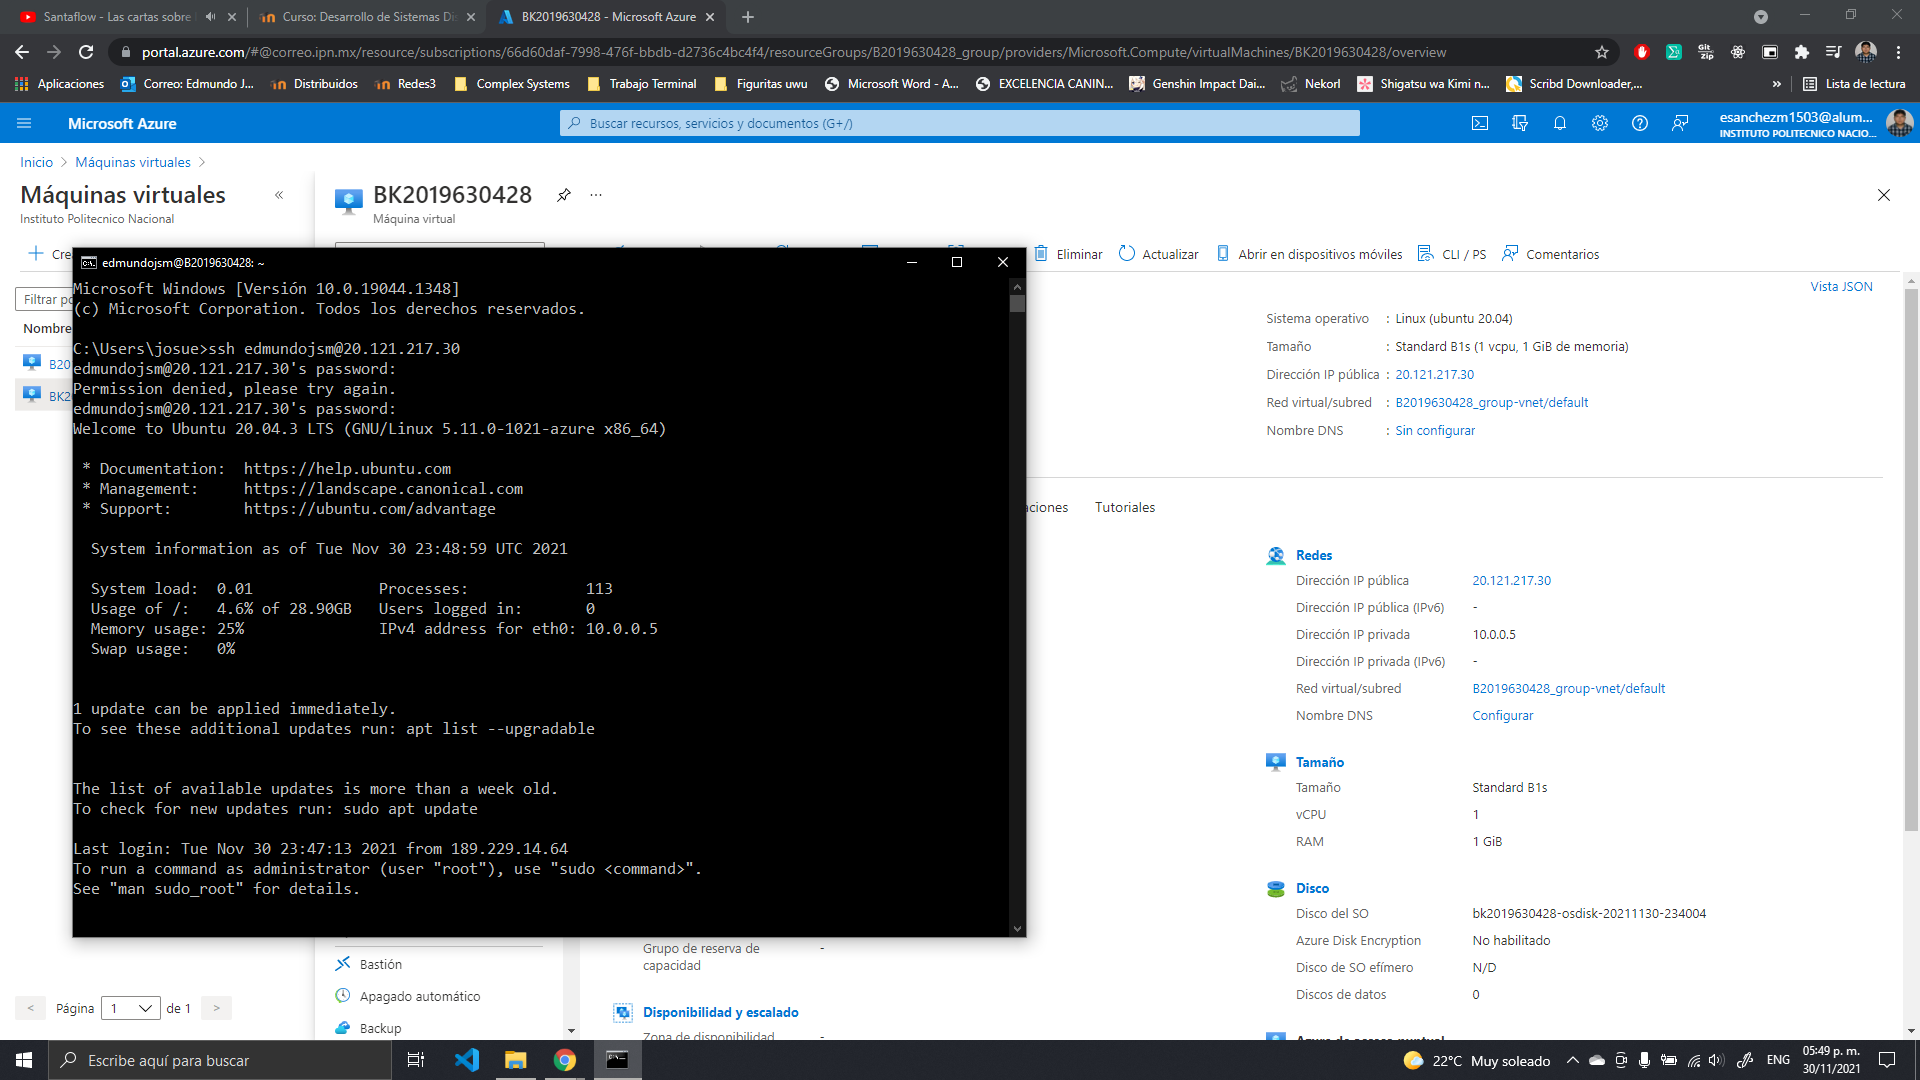
\includegraphics[scale=0.34]{resources/3.14.png}
			\caption{Conexión SSH a la nueva maquina virtual con las credenciales creadas para la maquina virtual inicial.}\label{fig:picture}
		\end{figure}
		Finalmente en la figura 26 podemos verificar que la configuración de la nueva máquina virtual es idéntica a la configuración de la máquina virtual respaldada.
		\begin{figure}[H]
			\centering
			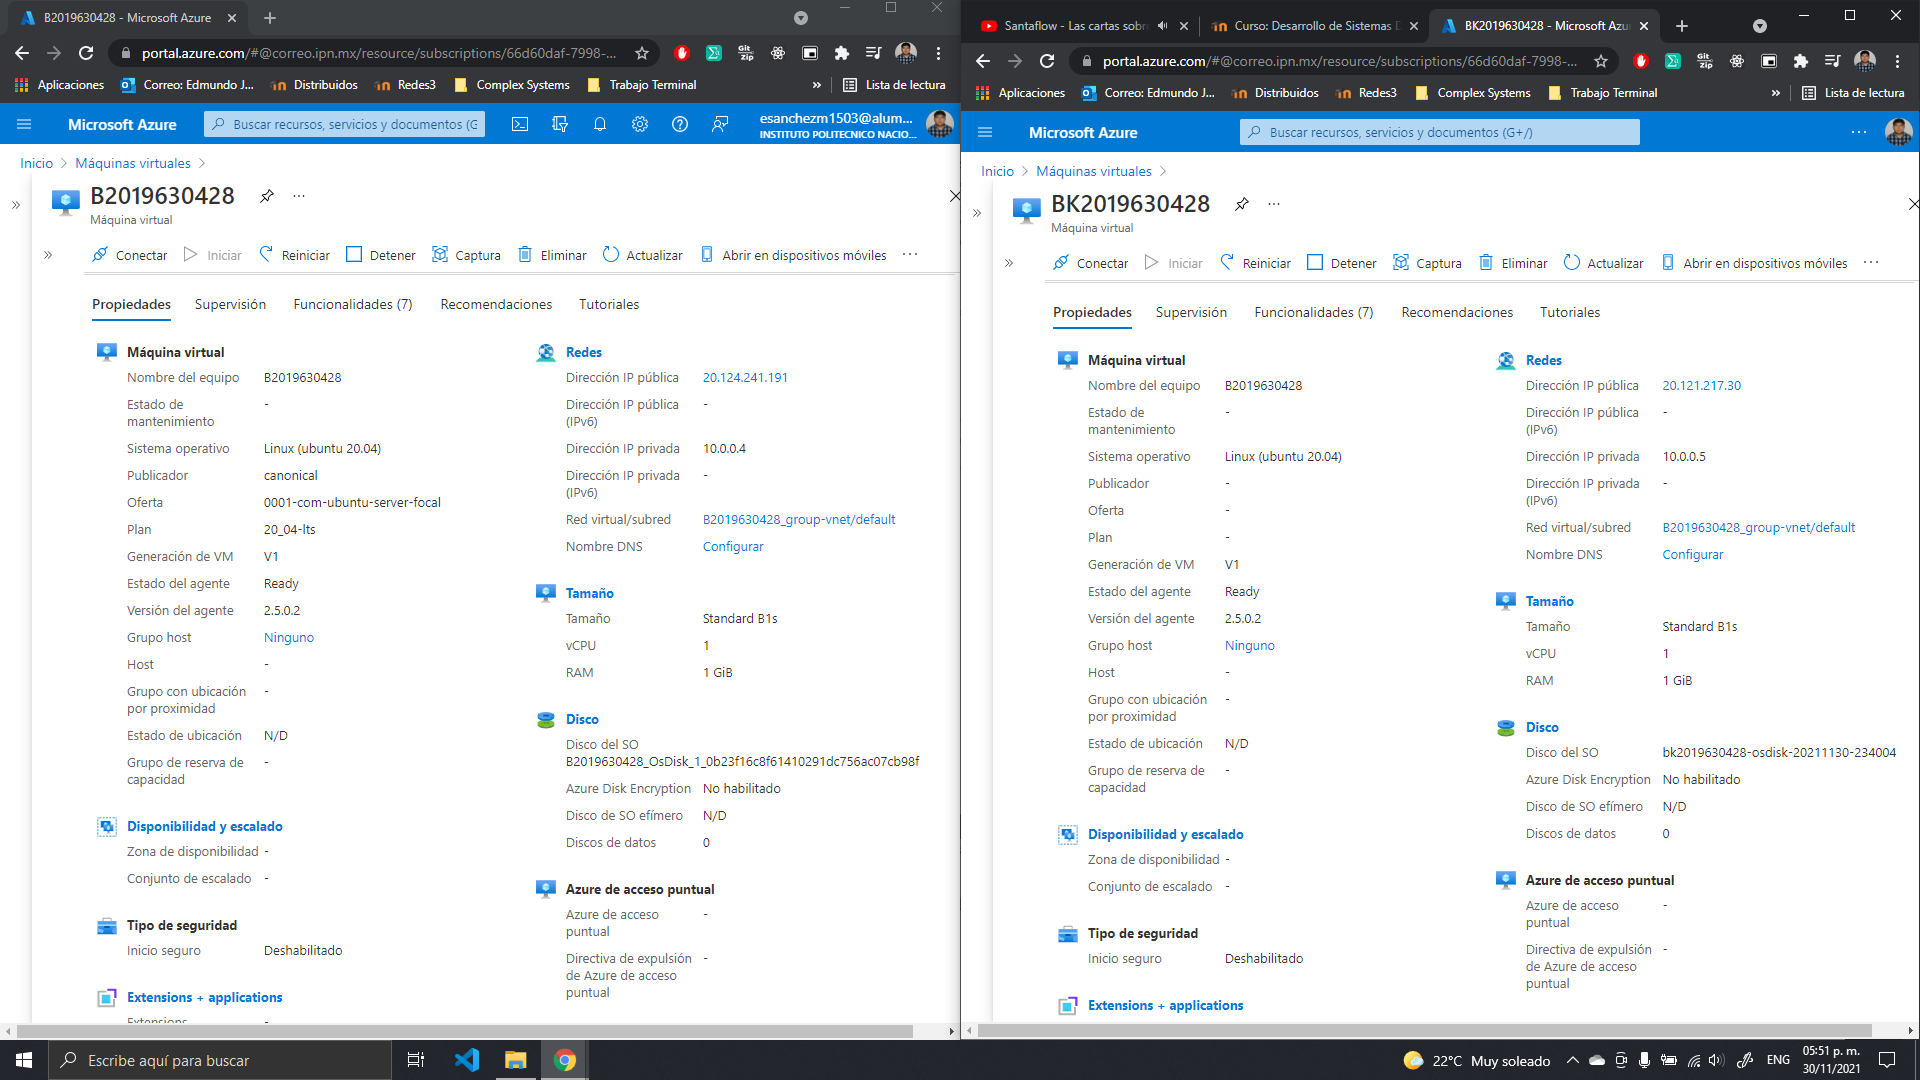
\includegraphics[scale=0.34]{resources/3.F.png}
			\caption{Configuración de la nueva máquina virtual es idéntica a la configuración de la máquina virtual respaldada.}\label{fig:picture}
		\end{figure}
		\subsection{Eliminar el proceso de respaldo}
		Para eliminar un proceso de respaldo y los puntos de respaldo asociados, debemos primero seleccionar la maquina virtual \textbf{INICIAL} e ir a la opción de ``Backup'' en el menú de ``Operaciones'', como vemos en la figura 27.
		\begin{figure}[H]
			\centering
			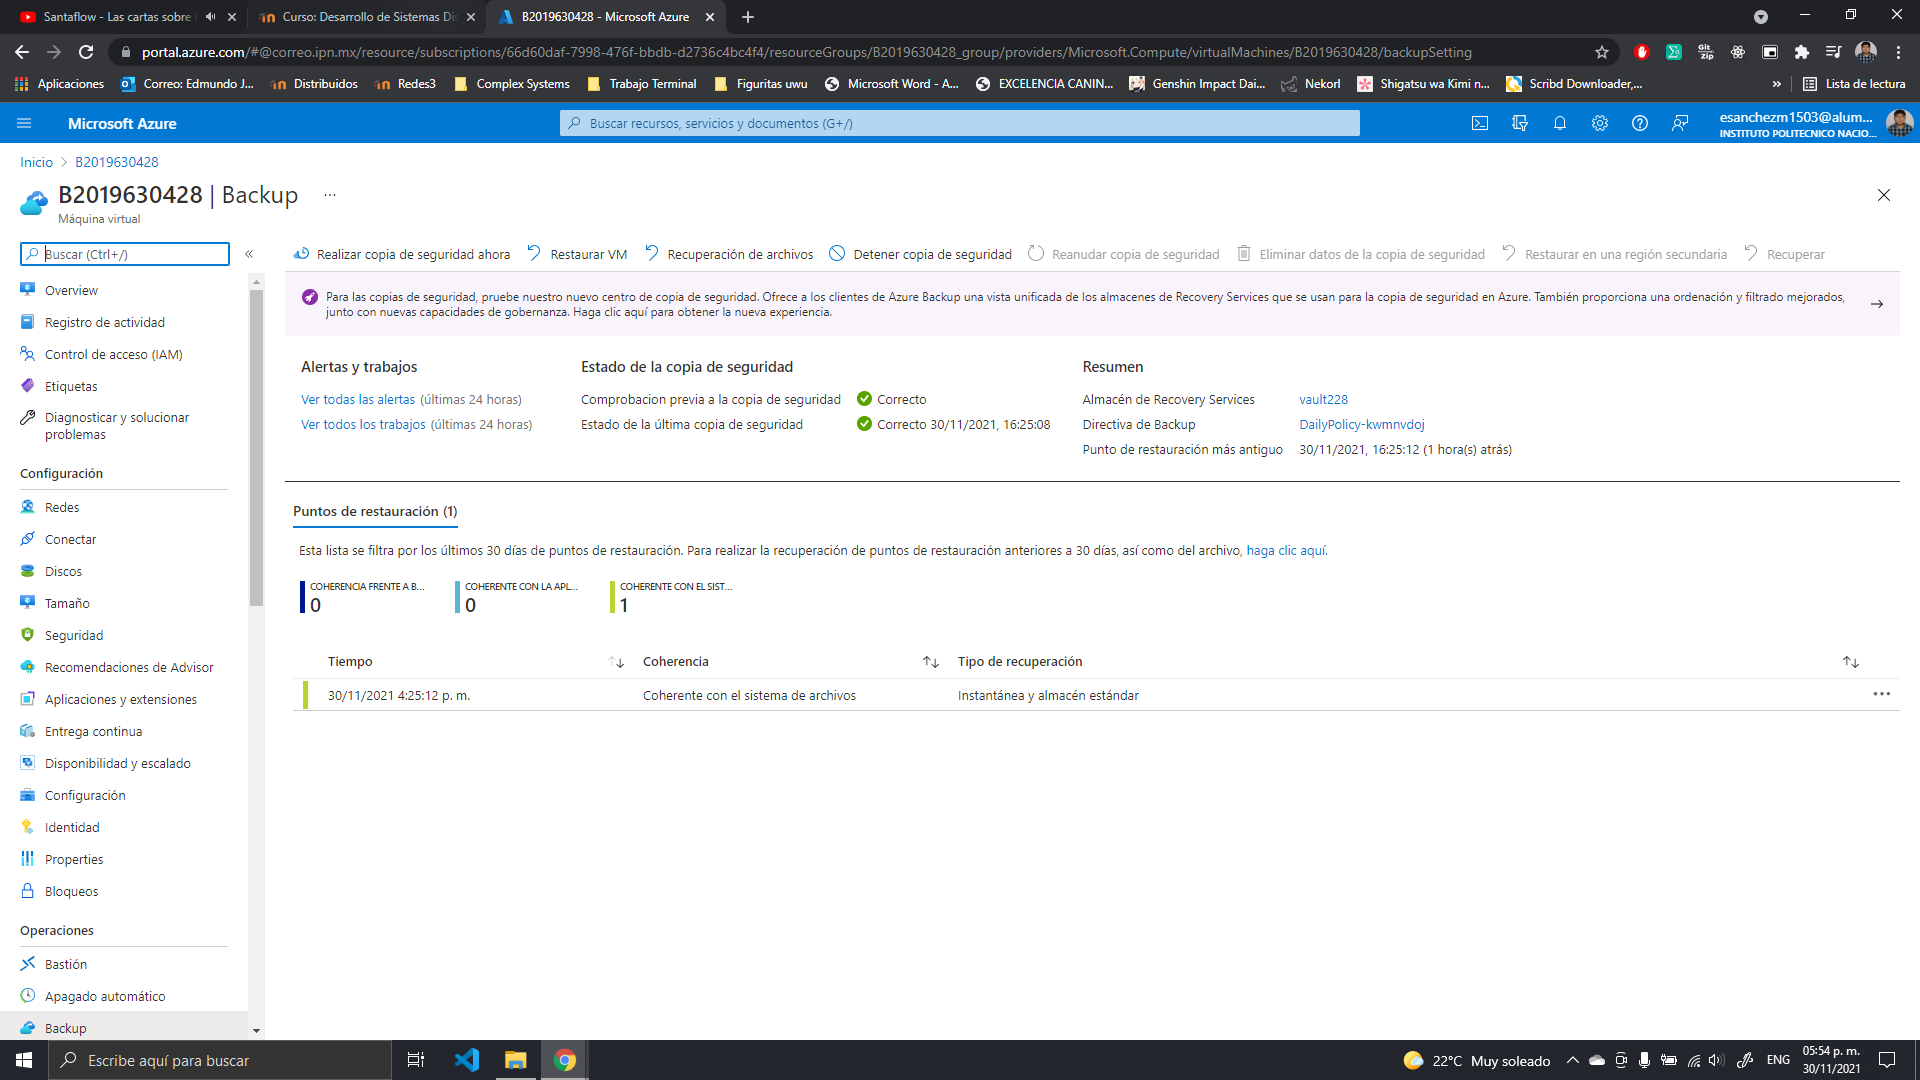
\includegraphics[scale=0.34]{resources/4.1-2.png}
			\caption{Opción de ``Backup'' en el menú de ``Operaciones'' de la maquina virtual inicial.}\label{fig:picture}
		\end{figure}
		Nos saldrá el formulario que podemos en la figura 28, ahí seleccionamos ``Detener copia de seguridad'', en caso de que no vea la opción presionar los tres puntos..., seleccionamos la opción ``Retener datos de copia de seguridad'' o bien ``Eliminar datos de copia de seguridad'', ingresamos el nombre del elemento de copia de seguridad, es este caso el nombre de la máquina virtual respaldada y opcionalmente se puede indicar el motivo por el cual se va a eliminar el proceso de respaldo. También es posible escribir algún comentario en la ventana ``Comentarios''.
		\begin{figure}[H]
			\centering
			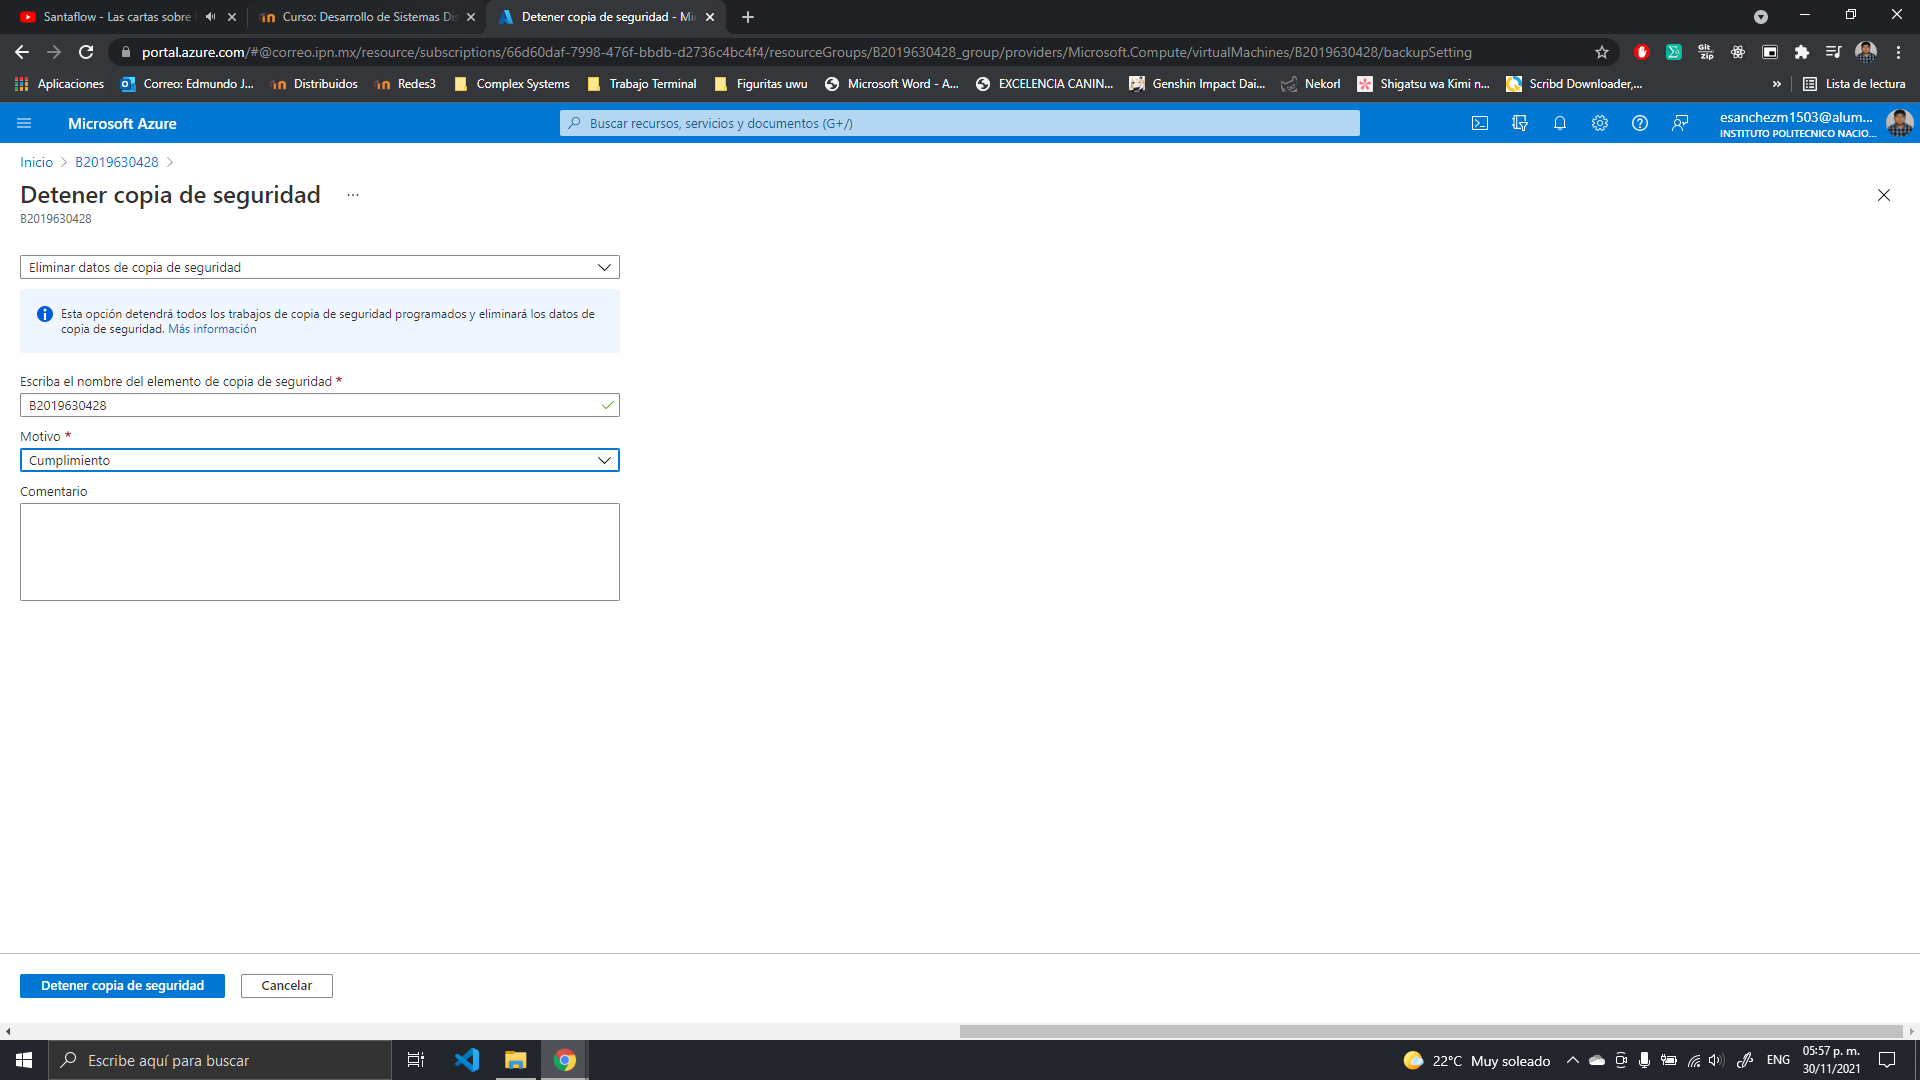
\includegraphics[scale=0.34]{resources/4.3-6.png}
			\caption{Eliminar el proceso de respaldo.}\label{fig:picture}
		\end{figure}
		 Daremos clic en el botón ``Detener copia de seguridad''. En la figura 29 damos clic en la campana de notificaciones para verificar que se haya detenido el proceso de copia de seguridad y en su caso, se haya eliminado los datos.
		 \begin{figure}[H]
			\centering
			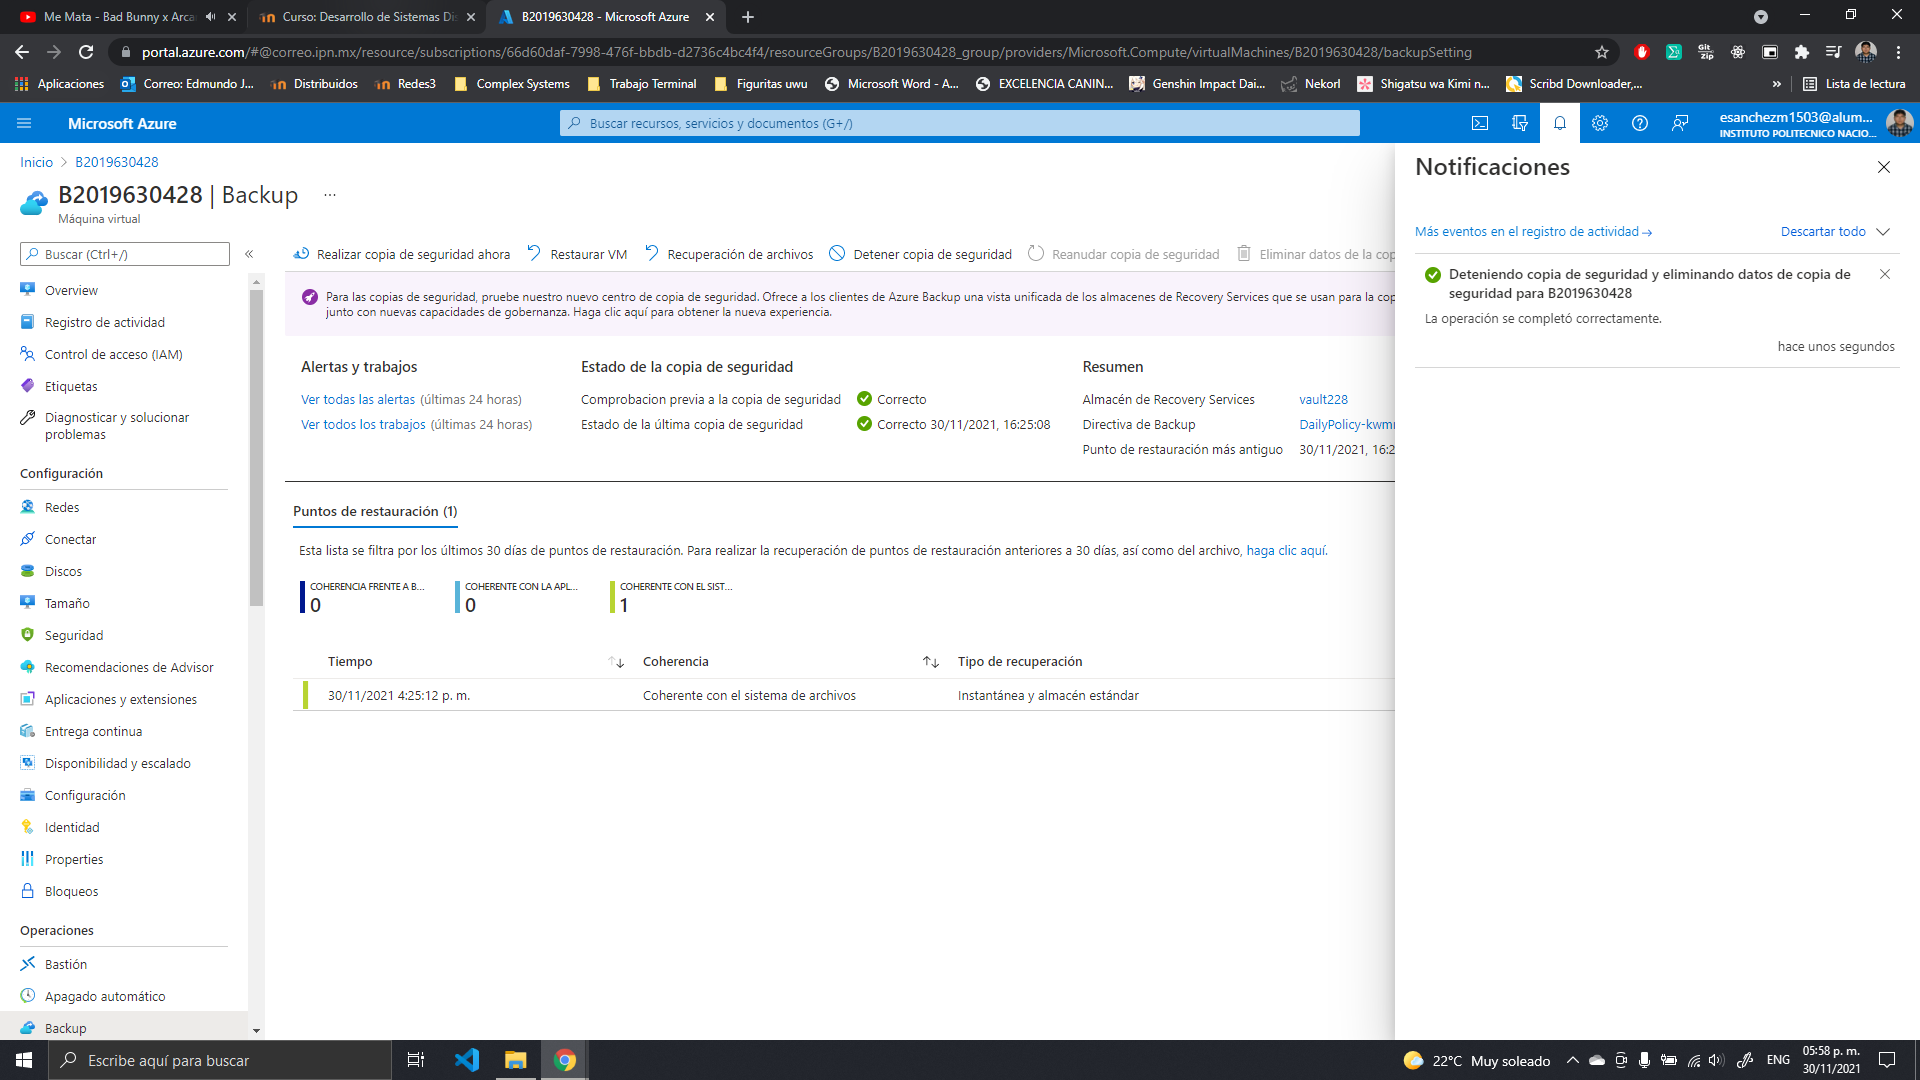
\includegraphics[scale=0.34]{resources/4.7-8.png}
			\caption{Proceso eliminado de manera exitosa.}\label{fig:picture}
		\end{figure}
		Finalmente hacemos una prueba de tratar de eliminar el almacén de Recovery Services (vault), para ello vamos a todos los recursos y seleccionamos el almacén creado en pasos anteriores como vemos en la figura 30 y en la figura 31 podemos ver como nos manda un mensaje de error de que no se pudo borrar ya que es necesario que hayan pasado 14 días desde el último respaldo, ya que la retención de los datos es por dos semanas, mencionar que este paso provoca un ``soft delete'' y es necesario hacer un proceso aparte para poder volver a usar este almacén, debemos de ir y seguir los pasos indicados en el siguiente enlace: \url{https://docs.microsoft.com/en-us/azure/backup/backup-azure-security-feature-cloud}.
		\begin{figure}[H]
			\centering
			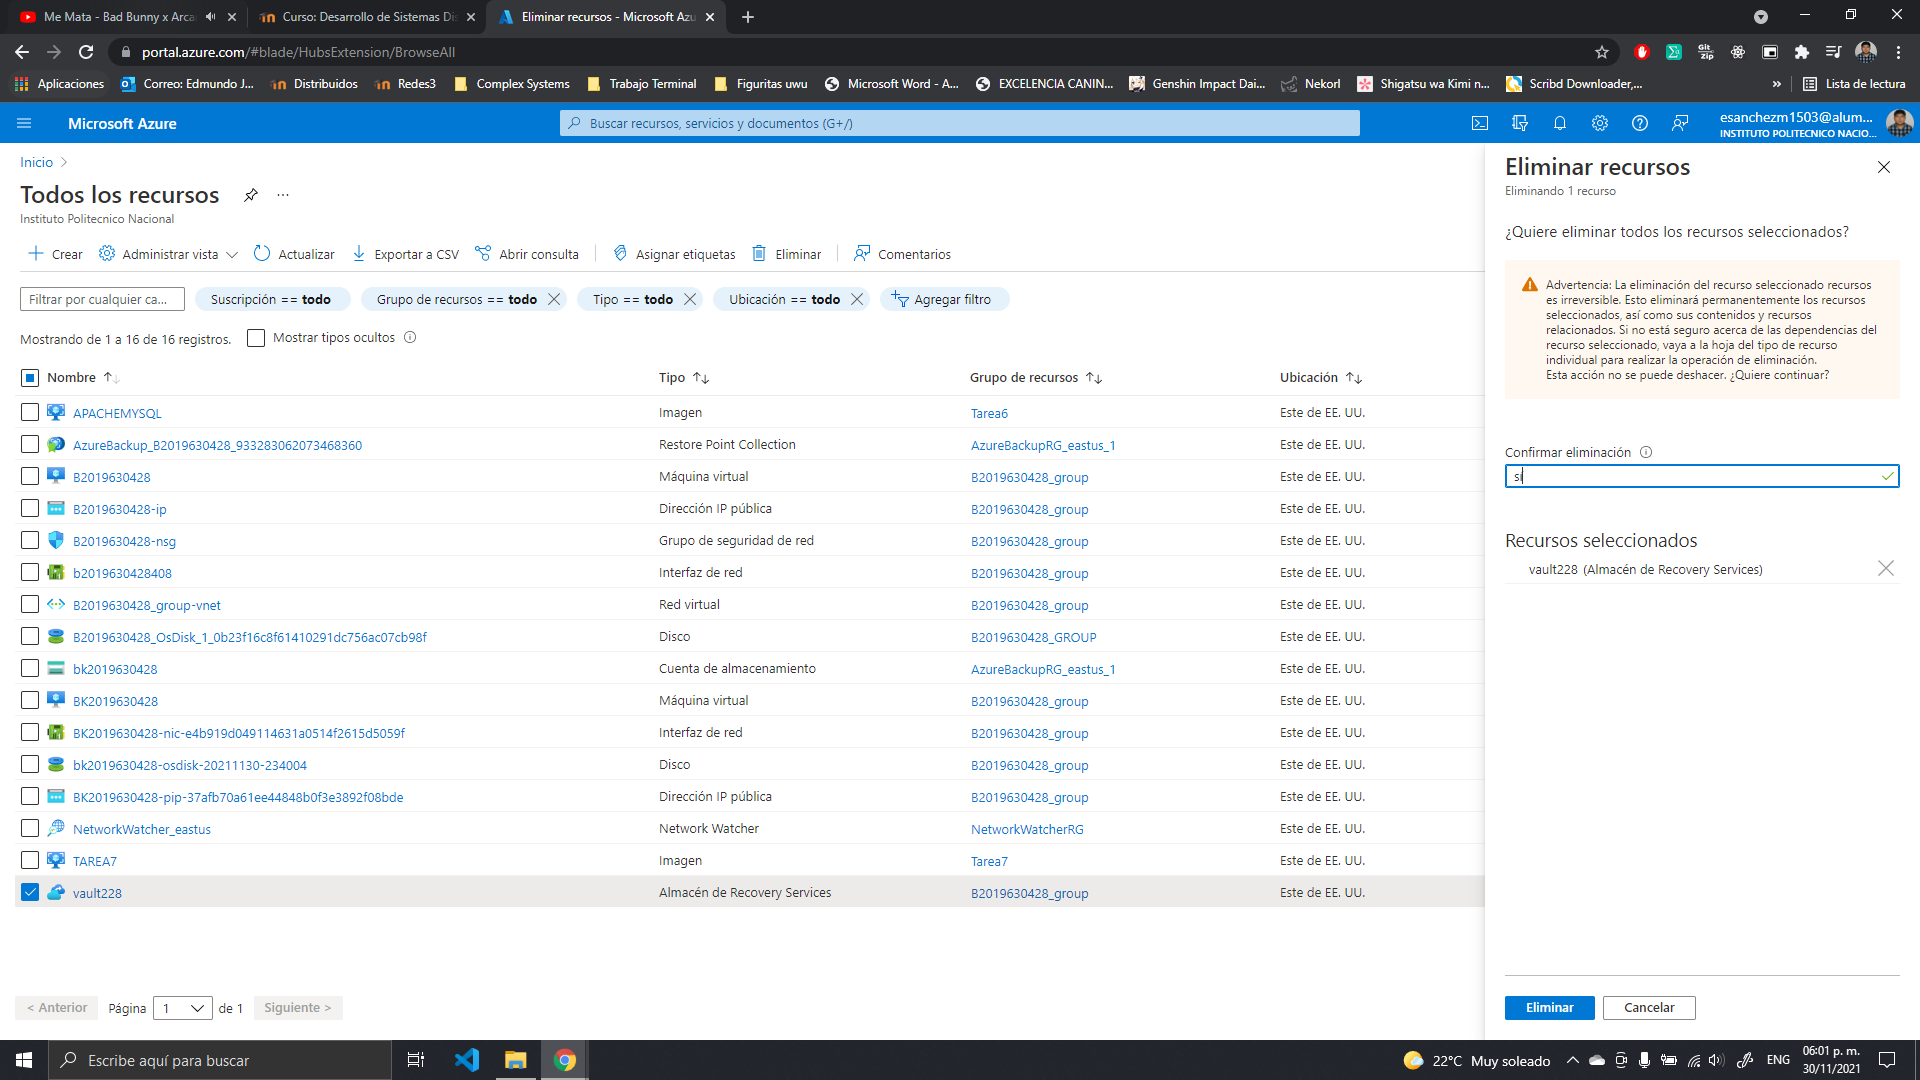
\includegraphics[scale=0.34]{resources/4.9.png}
			\caption{Intento de borrado del almacén de Recovery Services.}\label{fig:picture}
		\end{figure}
		\begin{figure}[H]
			\centering
			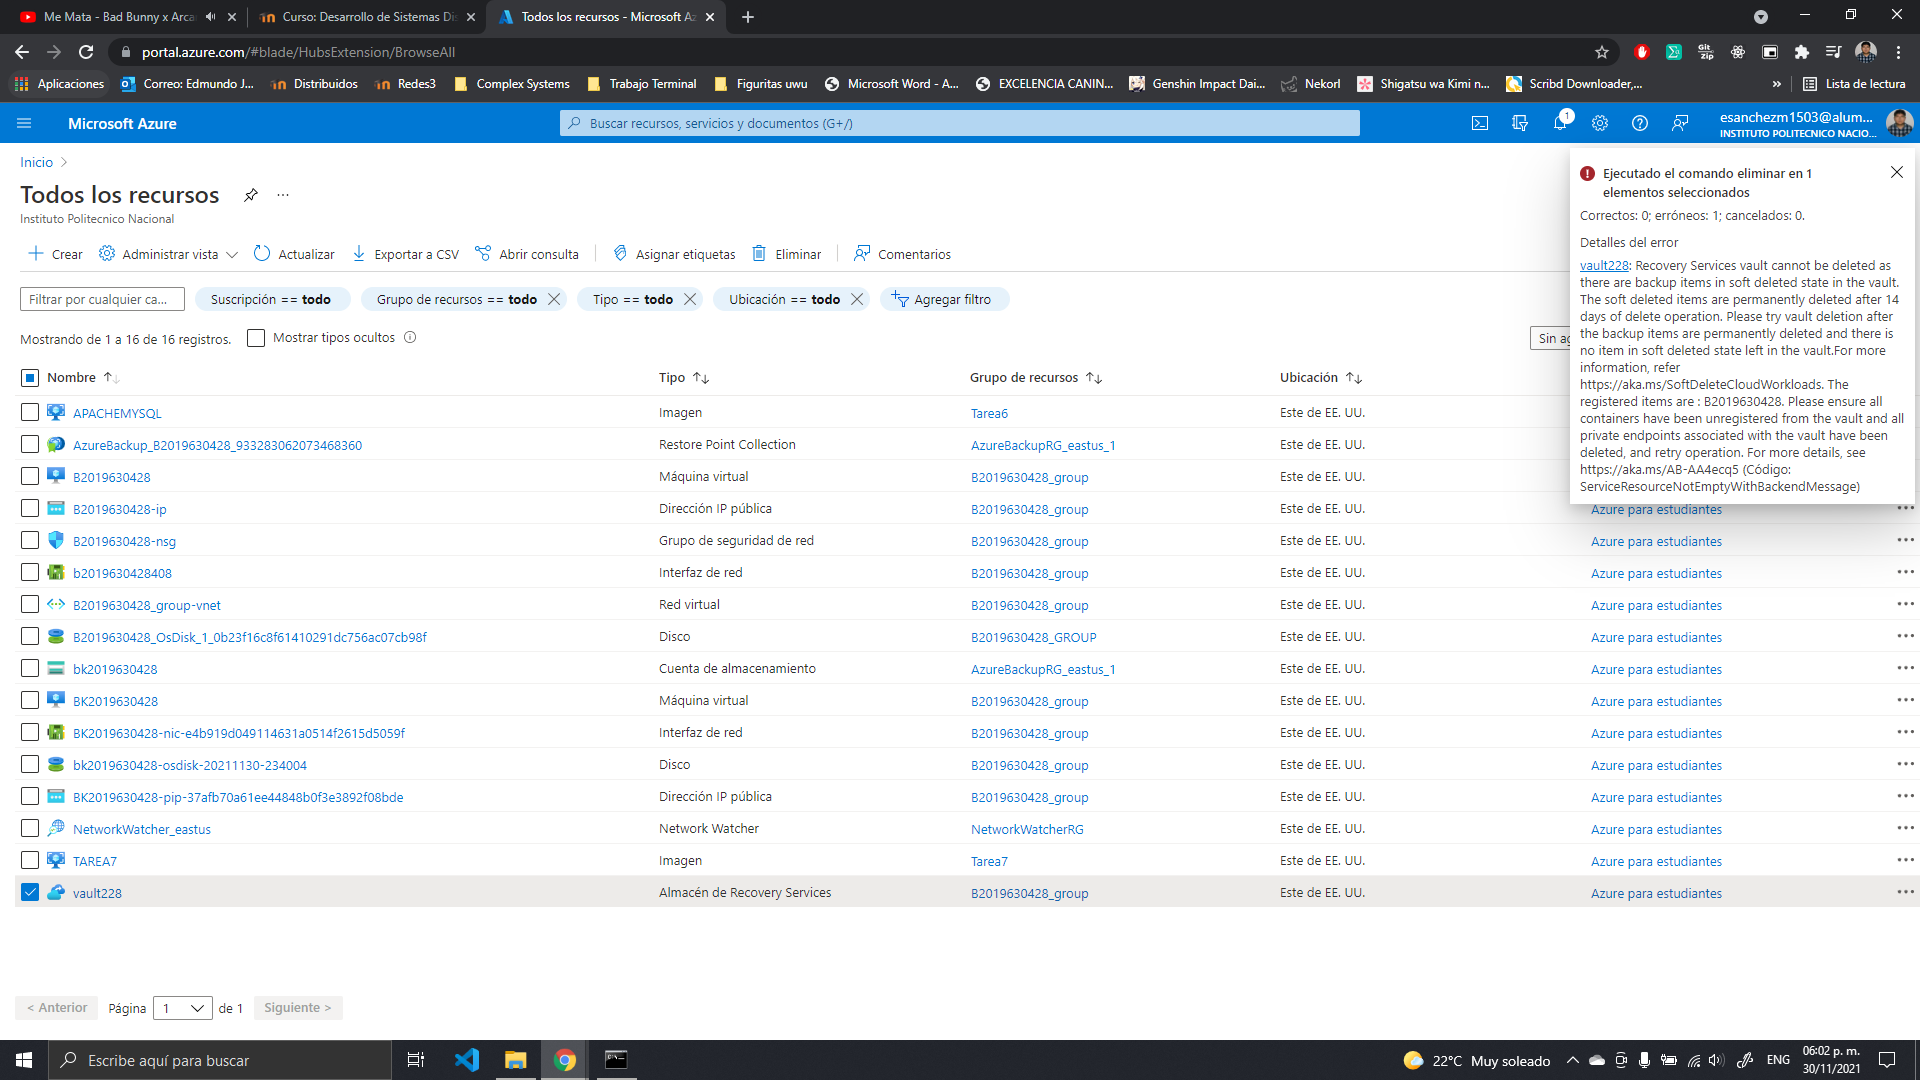
\includegraphics[scale=0.34]{resources/4.9error.png}
			\caption{Mensaje de error al intentar borrar el almacén de Recovery Services.}\label{fig:picture}
		\end{figure}
	\section{Conclusiones}
	En esta practica pudimos ver el servicio de Backup de Azure, el cual es un servicio de respaldo muy simple y amigable de usar y no es necesario tener conocimiento alguno sobre programación, de hecho cualquier usuario con los pasos que están presentes en este reporte lo podría llevar acabo. Sin embargo, es importante que el respaldo sea llevado por una persona de confianza o por nosotros mismo ya que respalda varias cosas, lo mejor de este servicio es que hace respaldos incrementales cada cierto periodo de tiempo, mencionar que el periodo lo podemos definir nosotros también. Finalmente comentar que es necesario considerar el tiempo que se tarda en realizar el respaldo ya que depende mucho del hardware de la maquina virtual, también comentar que esta tarea es útil en el campo laboral ya que muy probablemente en la empresa que se llegue a trabajar usen servicios en la nube y esto resulta muy útil.
		
\end{document}
